% Masterthesis 
% Rico Leuthold 2.9.2008
%
%noTeXShop

%---------------------------------------------------------------------------------------------------------
% Document setup
%---------------------------------------------------------------------------------------------------------

% paper format and stylesheet
\documentclass[a4paper,10pt,twoside,titlepage,headings=small,bibliography=totocnumbered,headsepline]{scrartcl}
\usepackage[bindingoffset=1cm,centering,includeheadfoot,margin=2cm]{geometry}
%\usepackage[english,german,brazilian]{babel}

% praphic package
\usepackage{graphicx}
\usepackage{wrapfig}

% used to change page setup
\usepackage{changepage}

% Font
\usepackage{times}
\usepackage[T1]{fontenc} 
\usepackage[english]{babel}
\usepackage{color}

% captions
\usepackage[format=plain,font=small,labelfont=bf,labelsep=period]{caption}

% orientation
\usepackage{rotating}
\usepackage{lscape}

%math
\usepackage{amsmath}

% used for citations
\usepackage[square, numbers, super]{natbib}

% Links
\usepackage[pdftex,hyperfootnotes=false,pdfborder=0 0 0]{hyperref}
\definecolor{darkgrey}{rgb}{0.2,0.2,0.2}
\hypersetup{
    colorlinks,%
    citecolor=black,%
    filecolor=black,%
    linkcolor=darkgrey,%
    urlcolor=blue
}

\urlstyle{rm}

% tables
\usepackage{tabularx}
\usepackage{ctable}
\usepackage{longtable}
%\usepackage{rotfloat}

% subfigures 
\usepackage{subfig}

% used for source code
\usepackage{listings}
\usepackage{fancyvrb}
\definecolor{lightgrey}{rgb}{0.95,0.95,0.95}

% appendix
\usepackage[toc,page]{appendix}

% heading on every page
\pagestyle{headings}

% Spacing
\frenchspacing

% Math symbols
\usepackage{mathabx} 

% ... some mor spacing stuff
\usepackage{setspace}


% border of pdf pics
\pdfpagebox 4

% Acronyms
\usepackage[printonlyused,withpage,footnote]{acronym}

% Space before and after paragraph title
\makeatletter
\renewcommand\paragraph{\@startsection{paragraph}{4}{\z@}%
  {-1.25ex\@plus -.5ex \@minus -.2ex}%
  {.5ex \@plus .2ex}%
  {\normalfont\normalsize\bfseries}}
\makeatother

%
% CUSTOM COMMANDS
%

% make inline listings normal font size
\makeatletter
\lst@AddToHook{TextStyle}{\let\lst@basicstyle\ttfamily\small\fontfamily{pcr}\selectfont}
\makeatother

% Code style with line numbers 
\newenvironment{numcodestyle}{
	\lstset{basicstyle=\footnotesize, numbers=left, numberstyle=\tiny, numbersep=3mm, stepnumber=1, backgroundcolor=\color{lightgrey}}
}

% Code style without line numbers
\newenvironment{codetiny}{
	\lstset{basicstyle=\tiny, numbers=none, backgroundcolor=\color{lightgrey}}
}

\newenvironment{codefoot}{
	\lstset{basicstyle=\footnotesize, numbers=none, backgroundcolor=\color{lightgrey}}
}

\newenvironment{codescript}{
	\lstset{basicstyle=\scriptsize, numbers=none, backgroundcolor=\color{lightgrey}}
}

% this makes description lists spacing much better.
\newenvironment{mydesc}{
	\begin{description}
	  \setlength{\itemsep}{1pt}
	  \setlength{\parskip}{0pt}
	  \setlength{\parsep}{0pt}
}
{
	\end{description}
}

% this makes description lists spacing much better.
\newenvironment{mylist}{
	\begin{itemize}
      \renewcommand{\labelitemi}{$\sqbullet$}
	  \setlength{\itemsep}{0pt}
	  \setlength{\parskip}{0pt}
	  \setlength{\parsep}{0pt}
}
{
	\end{itemize}
}


% this makes list spacing much better.
\newenvironment{condensed_enum}{
	\begin{enumerate}
	  \setlength{\itemsep}{1pt}
	  \setlength{\parskip}{0pt}
	  \setlength{\parsep}{0pt}
}
{
	\end{enumerate}
}

% this makes list spacing much better.
\newenvironment{condensed_item}{
	\begin{itemize}
      \renewcommand{\labelitemi}{$\circ$}
	  \setlength{\itemsep}{1pt}
	  \setlength{\parskip}{0pt}
	  \setlength{\parsep}{0pt}
}
{
	\end{itemize}
}

% Table column types for bold row 
\newcolumntype{+}{>{\global\let\currentrowstyle\relax}}
\newcolumntype{^}{>{\currentrowstyle}}
\newcommand{\rowstyle}[1]{\gdef\currentrowstyle{#1}%
#1\ignorespaces
}

%===============================
% Start document
%===============================
\begin{document}

% select language
\selectlanguage{english}

% Title page

\begin{titlepage}
\thispagestyle{empty}
\begin{flushleft}
\includegraphics[width=\textwidth]{assets/pdf/title_header.pdf}
\end{flushleft}
\vspace{3cm}
\begin{adjustwidth}{-.5cm}{-2cm}% adjust the L and R margins by 1 inch
\includegraphics[width=.8\textwidth]{assets/pdf/title_box.pdf}
\end{adjustwidth}
\vfill

\begin{figure}[htpb]% 
	\subfloat{
					\includegraphics{assets/pdf/title_author.pdf}
			}% 
	\hfill
	\subfloat{
					\includegraphics{assets/pdf/title_supervisor.pdf}
			} 
\end{figure}	 


%\includegraphics[width=\textwidth]{assets/pdf/title_footer.pdf}

\end{titlepage}

% Table of contents}
\tableofcontents
\listoftables
% add table of figures to toc
\listoffigures

% ===============================
% Introduction
% ===============================
% ===============================
% Introduction
% ===============================
\newpage

\section{Introduction}
\label{sec:introduction}

In May 2008, the research group around Prof. Barbara K\"onig at the Institute of Zoology of the University of Zurich decided to take their research in the field of Animal Behaviour to the next level. Especially interested in the complex social behaviour of house mice \textit{(Mus domesticus)} (see section \ref{subsec:socialbehaviour} on page \pageref{subsec:socialbehaviour} for details) they had the idea to design an automated system, to collect spatial position data of mice living in a shed.

\subsection{Motivation}
\label{subsec:motivation}
The motivation for such an effort is to obtain a statistically relevant set of data to develop, test and prove scientific thesis about the complex social behaviour of the house mice. The research interests are outlined in section \ref{subsec:researchtopics} on page \pageref{subsec:researchtopics}. An automated system has the advantage that it collects data 24 hours a day, and the mice are in no way disturbed in their natural behavior by the presence of men.

My personal motivation comes from the interest in informatics and my study in biology. The project gave me a lot of room to enhance my skills in informatics, while working on an interesting biological topic. Additionally I am interested in the \textit{network approach} to analyze complex social behaviour by the use of \textit{Graph theory}\cite{wiki:graph_theory}, which is outlined in section \ref{sec:netexp} on page \pageref{sec:netexp}.

The system collecting the data in the shed has been developed and constructed by \textit{New Behaviour}. For further information about the design and operation of the system please see section \ref{subsec:collectspatialpos} on page \pageref{subsec:collectspatialpos}. Thus, the main task for my master thesis was to provide tools to store the data and make it accessible to the users, which are mainly the researchers involved in the house mice project. 

\subsection{Task}
\label{subsec:task}
Handling the spatial position data collected by the automated system is challenging, as it includes several tasks which can be carried out only using informatics on a level that biologists normally can not cope with.

\subsubsection{Storing and Accessing the Data}
\label{subsubsec:storeaccess}
The sheer amount of data, expected to be collected by the automated system, has to be stored in a secure and stable way. The only reasonable way to fulfill these conditions, is to set up a \ac{RDBMS} (RDBMS) (see section \ref{subsec:datastorage} on page \pageref{subsec:datastorage}). 

To access the data, an intuitive user interface must be available, which facilitates the data exploration and export (see section \ref{subsec:dataccess} on page \pageref{subsec:dataccess}). The technology used to create the interface should be cross-platform compatible.   

\subsubsection{Additional Tasks}
\label{subsubsec:additional}
Additionally, the user should be provided with an interface to administrate attribute data, such as the sex of the mice (see section \ref{subsec:dataattr} on page \pageref{subsec:dataattr}) and to carry out some simple data analysis methods.

Last but not least, some functionality should be present which allows the user to compile data for a possible analysis according to the network approach (see section \ref{sec:netexp} on page \pageref{sec:netexp}).

% ===============================
% Biology of the house mice
% ===============================
% ===============================
% Biology of the house mice
% ===============================
\newpage
\section{Biology of the house mouse}
\label{sec:biolhousemice}

\subsection{Introduction}
\label{subsec:introduction}

House mice (\textit{Mus domesticus}) (see figure \ref{fig:housemice}) live under a multitude of different environmental conditions. The ecological success of house mice as a widely distributed species reflects the fact, that they are very flexible in terms of their social, territorial and reproductive behavior \citep{bronson:79, bronson:84, berry:81}. Under natural conditions house mice have a relatively low expectancy of life (100 to 150 days). During this short life span, female mice are avid to have as many offspring as possible. Living under optimal food conditions, a female mouse gives birth to a litter of 5-7 pups every four weeks \citep{berry:71, pelikan:81}. The juvenile mortality is estimated between 50\% and 85\% \citep{berry:71, berry:75, pennycuik:86}. Having heavier pups is an advantage, as they can be weaned faster, which positively influences future reproduction of the mother\citep{fuchs:82}. The litter size of a wild house mouse increases from the first to the second lactation and decreases after the fifth lactation \citep{pelikan:81, koenig:87b}. 

\begin{figure}[htbp]	
\centering	
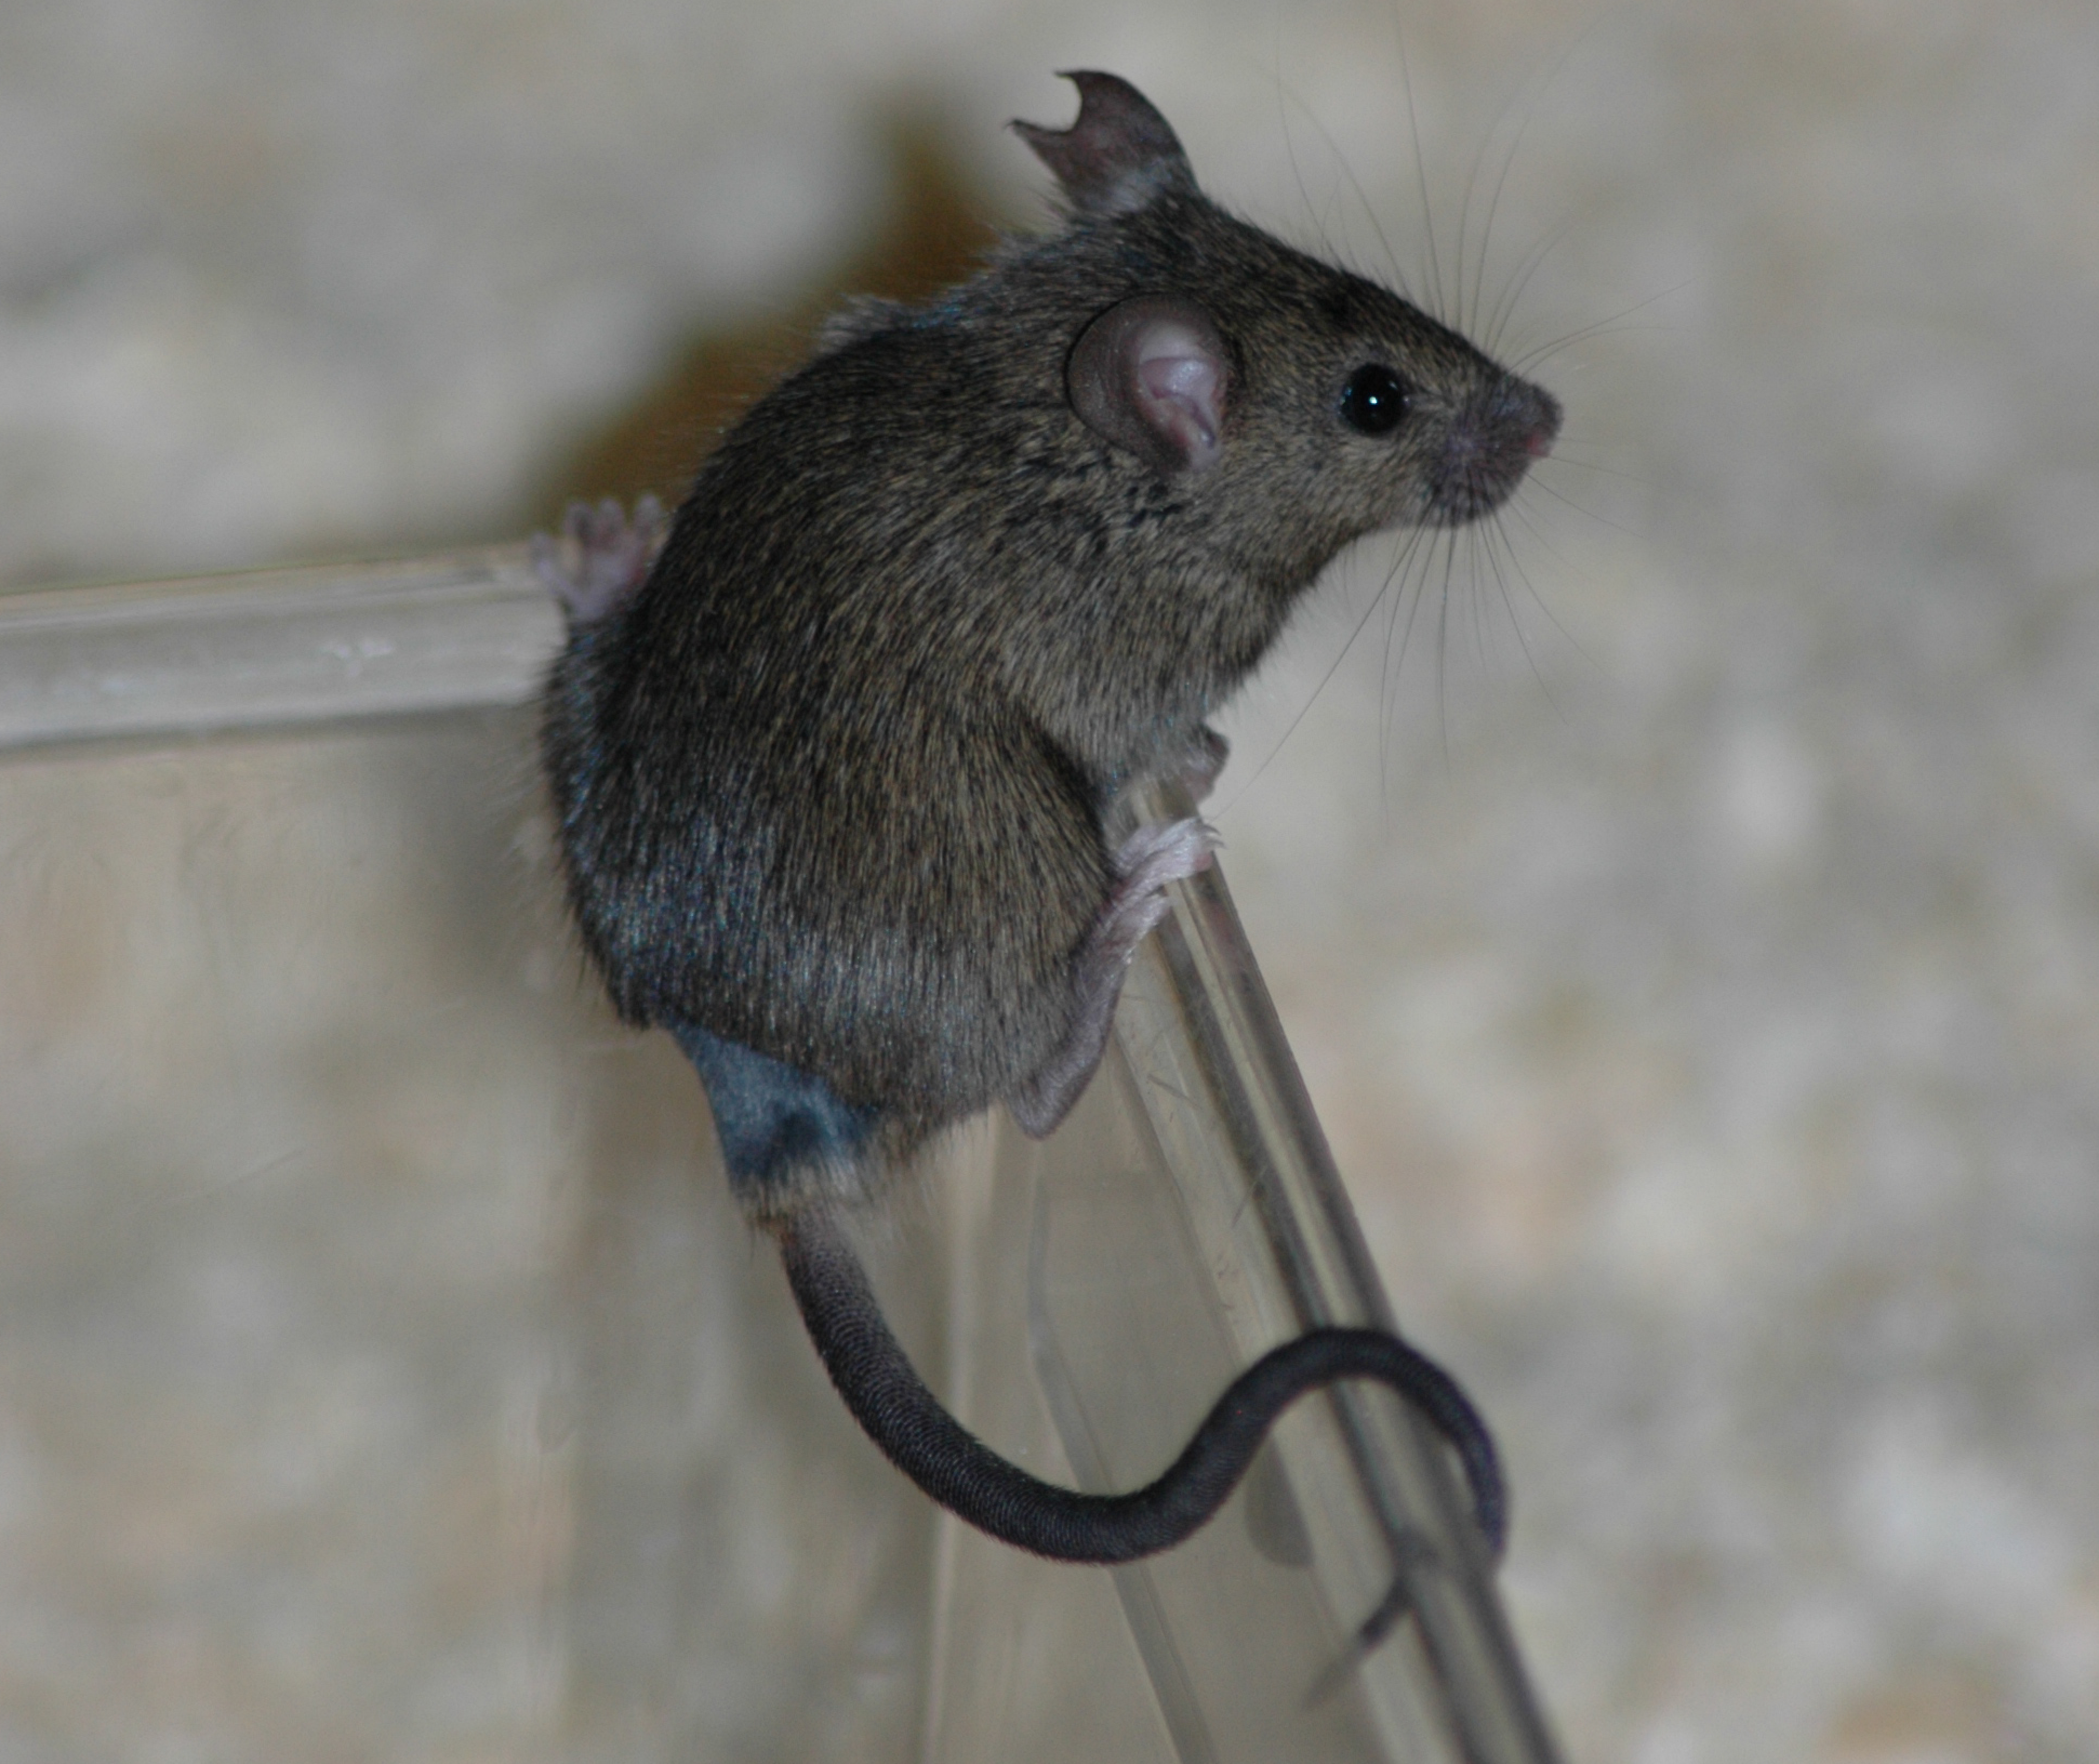
\includegraphics[width=0.5\textwidth]{assets/pdf/mus_domesticus.pdf}	
\caption[House mouse]{House mouse \textit{(Mus domesticus)}}
\label{fig:housemice}
\end{figure}

\subsection{General social behavior}
\label{subsec:socialbehaviour}
House mice typically live in a social collective which forms a reproduction group. These groups usually include a dominant male, one or several females with their litters and possibly some subordinate males \citep{crowcroft:63, reimer:67, selander:70, mackintosh:81}.

The mating habit is typically polygynandric (both males and females have several mating partners), but monogamic living pairs have also been reported \citep{lidicker:76}. Juvenile females may stay in the territory of their parents to raise their own offspring \citep{petras:67}. There is evidence of stranger females immigrating into social groups as well \citep{anderson:65, reimer:67, selander:70, bronson:79, baker:81}.     

\subsection{Research topics}
\label{subsec:researchtopics}

The research group in animal behavior around Prof. K\"onig at the University of Z\"urich is generally interested in the complex social behavior of the house mice. Mainly the influence of the social partner choice, other then mating, onto the fitness of the female mice, is in the focus of the studies. Such social selection occurs, if social interactions result in favorable fitness consequences. Therefore, reproductive cooperation such as joint nesting, for example, should manifest in an increased number of offspring \citep{weidt:07}. Cooperative interactions can extend to sharing of broad-rearing duties like nursing.

\subsubsection{Communal nursing}
\label{subsubsec:comnurs}

Over forty years ago, first observations of wild female house mice, belonging to the same reproduction group, which raise their pups in communal nests have been reported \citep{southwick:55}. Ever since, this behavior has been noticed for house mice living under all kind of environmental conditions.\citep{crowcroft:63, sayler:69, gandelman:70, werboff:70, baker:81}.

This behavior is astonishing, as the energetic costs of lactation are very high, hence influence the females' future reproduction success. To wean a litter of about seven to eight pups, the mother has to produce 100 grams of milk within 22 days, which is equivalent to 1100 \acf{KJ} \citep{koenig:88}. Depending on the size of the litter and the duration of the lactation phase, the length of the interbirth intervals change \citep{fuchs:81, fuchs:82, koenig:87a, koenig:87b}.

Several experiments have been carried out with wild house mice living under laboratory conditions. Manipulating group size and the composition of the group in terms of relatedness of the individuals revealed that non-offspring nursing is an integral part of the reproductive behavior of female house mice in egalitarian groups. However, the probability for such mutualistic cooperation was highest when a female shared a nest with a familiar sister to form a low-skew society \citep{koenig:06}.

According to K\"onig \citep{koenig:06}, the direct benefits of allomaternal care for the pups could be diverse. As there are, improved survival, improved future reproduction, improved growth or immunological benefits.

There are physiological benefits for the mother as well, which lead to an increase of their reproductive output. Of notable interest is the hypothesis named \textit{Metabolic peak load reduction}. Explained in short, a solitary nursing female tends to have a peak of energy consumption during the nursing phase of her litter. Nevertheless, female house mice are limited in their maximal sustainable metabolism \citep{hammond:92}. This limit depends on the age and physique of the individual and is called \textit{metabolic ceiling}. Partial synchronization in reproduction within the females of a group, combined with the communal nursing, can balance the energy demand for the individual, as the burden of nursing the litter is divided. Hence, the energy demand for each female stays always on a medium level\citep{koenig:06}. This can result in an increased lifetime reproduction success.

However, due to the artificial setup of the experiments, no conclusion about the communal nursing under natural conditions could be made.


% ===============================
% Shed setup
% ===============================
% ===============================
% Shed setup
% ===============================
\newpage
\section{Experiment set-up}
\label{sec:shedsetup}

Since 2003 the K\"onig lab studies a wild population of house mice in a barn, where mice can leave and enter as they wish.

The barn is located in a forest near Illnau (Switzerland) and consist of a single room with an area of 64m$^2$ (12.8m x 5.75m). Stable plastic walls (height \textasciitilde50cm) divide the area into four segments and an entry space. Small transit holes in the dividers ensure access to the different segments (see figure \ref{fig:shedschema}).

The entry area provides workspace for the researchers and is used to store tools and material. Furthermore, the central computer for the data collection system (see section \ref{subsec:collectspatialpos}) is placed in this area.

The 40 artificial nestboxes (see figure \ref{fig:artNestbox} for a schematic model) are distributed evenly in the four sectors (see figure \ref{fig:shedschema} for the current positioning of the boxes) along with some plastic pipe structures, bricks, smaller plastic walls and shelters to structure the environment (see figure \ref{fig:shedoverview}). These structuring elements ensure the existence of several territories, and provide hideouts for the subordinate mice.

\begin{figure}[htpb]
\begin{center}
  \includegraphics[width=0.7\textwidth]{assets/pdf/shed_overview.pdf}
  \caption[Interior of the barn]{Overview of the interior of the barn. Visible are the artificial nestboxes labeled with the box number on the white cover panel, the grey colored sector dividers and the accessory elements to structure the area.}
  \label{fig:shedoverview}
\end{center}
\end{figure}

\begin{sidewaysfigure}[htpb]
  \includegraphics[width=\textwidth]{assets/pdf/shed_schema.pdf}
  \caption[Schema of the barn]{Schema of the barn including the box positions and the plastic walls dividing the area in the four segments. }
  \label{fig:shedschema}
\end{sidewaysfigure}

% ===============================
% Data collection
% ===============================
% ===============================
% Data collection
% ===============================
\newpage
\section{Data}
\label{sec:datacollection}

When gathering data for behavioral analysis of different species, the observer usually tracks the position of one or several individuals over time. Additionally, pheno- and genotypical data is collected about each individual.

Spatial position is usually recorded by one or several persons. In this project however, data is collected by an antenna system (see section \ref{subsec:collectspatialpos}). Obviously, automated data collection has the advantage that data is recorded automatically around the clock every day.

To collect phenotypical data, so called \textit{population checks} (see \ref{subsec:dataattr} on page \pageref{subsec:dataattr} for details) are conducted every 6 to 8 weeks. During these checks, the mice are caught, measured, weighed (see section \ref{subsec:dataattr}) and - if not already present and the mouse has a weight of at least 18 grams - a \ac{RFID} (RFID) transponder is injected hypodermically (Figs.\ref{fig:transponder} and \ref{fig:inject_rfid}). About 240 transponders are injected every year.

\begin{figure}[htpb]
\begin{center}
\includegraphics[width=0.5\textwidth]{assets/pdf/transponder.pdf}
  \caption[Trovan ID-100A Microtransponder]{A Trovan ID-100A Microtransponder. The transponder weighs 0.1 g and is coated with biocompatible glass. \footnotesize Picture courtesy of Trovan.}
  \label{fig:transponder}
\end{center}
\end{figure}
\begin{figure}[htpb]
\begin{center}
\includegraphics[width=0.5\textwidth]{assets/pdf/transponder_inject.pdf}
  \caption[Subcutaneous injection of an RFID transponder]{Subcutaneous injection of an RFID transponder.}
  \label{fig:inject_rfid}
\end{center}
\end{figure}

Furthermore, tissue samples are taken from the ear of each individual for genetic analysis. The genetic information provides an insight into the relatedness within the mice population and allows to compare specific genetic markers. Genotype information is not included in the data used for this thesis.

%----------------------------------------------
%Position / Time data
% ----------------------------------------------
\subsection{Collecting spatial position data}
\label{subsec:collectspatialpos}

To collect the spatial position data, a project-specific system has been by built by \textit{NewBehavior}, a company specialized in developing technical systems to study animal behavior.

The basic idea is to identify mice carrying an RFID transponder at specific locations. The locations where the identification occurs are the 40 artificial nestboxes distributed in the barn. 

An artificial nestbox consists of a cylinder, made of \ac{PVC}, with diameter and height of 15 cm and an entry tube made of \textit{Plexiglas}, which is about 20 to 25 cm long. Wrapped around the tube are two antennas with a coverage radius of 10 to 12 cm, capable of reading out the RFID transponders. Each antenna can be identified by an address which is set manually. To improve the antenna accuracy, the entry tube is bent 45 degrees to slow down the mice passing through. Figure \ref{fig:artNestbox} depicts a model of such an artificial nestbox.

\begin{figure}[htbp]	
\centering	
\includegraphics[width=\textwidth]{assets/pdf/box_schema.pdf}	
\caption[3D-Model of an artificial nestbox]{3D-Model of an artificial nestbox with the two antennas wrapped around the entry tube.}
\label{fig:artNestbox}
\end{figure}

The RFID transponders used are passive, meaning that they do not include a battery. The antenna acts as a scanner, presenting an inductive field that excites the transponder within antenna range. This energy is used by the transponder to send its identification to the antenna. 

Therefore, whenever a mouse carrying a transponder passes by an antenna, its identification is recorded and sent to a central computer along with the antenna address. The computer then adds a time value to the received data before writing it to a text file. The structure of these text files containing the data is detailed in the next section.

\subsubsection{Data file format}
\label{subsubsec:datafileformat}
The data files are simple text files, where each line denotes an event registered by an antenna in the system. Every day the data file is saved, closed, and a new one is created automatically by the system.

There are two types of events: %Bullets! -tnetter 09/09/2009 15:35 % rico - how do put that in a list without a point at the end? 
\begin{mylist}
 \item The first type occurs if the antenna could identify a transponder. In such a case a line as shown in figure~\ref{fig:dataset} is written to the data file. The id of the transponder is a unique, ten character wide, alphanumeric value,
 \item The second type of event, for which the resulting data line looks as shown in Fig. \ref{fig:dataset_no_data}, occurs when a transponder enters or leaves the coverage area of an antenna.

\end{mylist}

\begin{figure}[!htbp]	
\centering	
\includegraphics[width=0.6\textwidth]{assets/pdf/dataset.pdf}	
\caption[Dataset including an RFID transponder identification]{Typical dataset in a data file including an RFID transponder identification.}
\label{fig:dataset}
\end{figure}

\begin{figure}[!htbp]	
\centering	
\includegraphics[width=0.6\textwidth]{assets/pdf/dataset_no_data.pdf}	
\caption[Dataset without RFID transponder identification]{Typical dataset in a data file without an RFID transponder identification.}
\label{fig:dataset_no_data}
\end{figure}

\needspace{9\baselineskip}
The following clipping and corresponding list show the data generated when a transponder passes by a nestbox. The events are explained in the subsequent list.  

\numcodestyle
\begin{lstlisting}[frame=none]
2008-10-01 16:31:08:499;   111;   0; 
2008-10-01 16:31:09:095;   113;   0; 
2008-10-01 16:31:42:512;   111;   5;  00 06 B8 D4 5A
2008-10-01 16:31:42:807;   113;   5;  00 06 B8 D4 5A
2008-10-01 16:31:43:619;   111;   0; 
2008-10-01 16:31:44:014;   113;   0;
\end{lstlisting}

The list numbering matches the line numbering of the clipping.  

\begin{condensed_enum}
  \item Transponder \textbf{enters coverage area} of the antenna with address \lstinline|111|.
  \item Transponder \textbf{enters coverage area} of the antenna with address \lstinline|113|.
  \item Transponder is \textbf{identified} as \lstinline|00 06 B8 D4 5A| at antenna with address \lstinline|111|.
  \item Transponder is \textbf{identified} as \lstinline|00 06 B8 D4 5A| at antenna with address \lstinline|113|.
  \item Transponder \textbf{leaves coverage area} of the antenna with address \lstinline|111|.
  \item Transponder \textbf{leaves coverage area} of the antenna with address \lstinline|113|. 
\end{condensed_enum}

Depending on the event type, the value of the packet size is either a \lstinline|0|, for events without a transponder identification value, or a \lstinline|5| if the transponder has been identified. For the data processing (see section \ref{sec:dataproc} on page \pageref{sec:dataproc}) only the datasets with a transponder identification are taken into account.

\subsubsection{Antenna addressing}
\label{subsubsec:addressing}

The antenna address is three digits long, composed of the box number it is attached to (first two digits) and the position at the entry tube of the box. Outer antennas have a \lstinline|1| as the last digit of the address, inner antennas a \lstinline|3| (e.g the antennas attached to box 11 are addressed 111 for the outer, 113 for the inner antenna, respectively). Needless to say, box numbers must be unique.

Unfortunately there are a few exceptions to that schema, as for a few antennas the correct addressing failed due to technical problems (see section \ref{subsec:problems}).

% \subsubsection{General system design and functionality}
% \label{subsubsec:generalsystem}
% 
% \begin{itemize}
%   \item Can-Bus
%   \item cable loop
%   \item rfid identification how
%   \item What happens in the boxes (boards) next to the antennas
%   \item How is can bus working/implemented
%   \item Where are the different cable loops (which antennas connected to a loop)
%   \item General system layout (cabling, protocols)
%   \item Programmed software
%   \item etc. 
% \end{itemize}

% ----------------------------------------------
%Data attributes
% ----------------------------------------------
\subsection{Collecting Data Attributes}
\label{subsec:dataattr}

During the \textit{population checks}, the whole barn, including all nestboxes, plastic pipes, and other structuring elements, is checked to collect mice attribute data according to the following procedure:

\begin{enumerate} 
\item Each box is opened and the following observations made:
\begin{mylist}
      \item \textbf{Mice in the box:} If adult mice are in the box, they get identified by their transponder, measured, and weighed. Furthermore we check whether the sex of the mouse has already been determined.  
      \item \textbf{Bedding:} Determine if the nestbox shows marks of use, like trampled bedding.
      \item \textbf{Nest:} Determine whether the nestbox contains an open or closed nest built by the mice out of hay or straw regularly provided in the barn.  
      \item \textbf{Pups:} Does the box contain pups, and if yes how many and what is their estimated age. 
      \item \textbf{Communal nest:} Check if two or more litters are reared in the box. 
    \end{mylist}
\item All the possible shelters, like planks and pipes, are checked for mice presence as well.
\end{enumerate}

% ----------------------------------------------
%storing Data
% ----------------------------------------------
\subsection{Data storage}
\label{subsec:datastorage}

This section details the design of the database. Data is stored in a \textit{MySQL}\footnote{\href{http://www.mysql.com/}{MySQL database}} database, which is  a \acf{RDBMS} (RDBMS). Figure \ref{fig:database_schema} on page \pageref{fig:database_schema} in the appendix shows an overview of all tables, including the data types\footnote{An overview of the MySQL data types can be found at: \url{http://dev.mysql.com/doc/refman/5.0/en/data-types.html}} of the columns and their relationship to columns in other tables.

Upon completion of a cascade of \ac{perl} scripts that process and extract information from the spatial position data in the data files, the resulting data is merged with the collected attribute data and is written to the tables as outlined in here. For details about the cascade refer to section \ref{sec:dataproc}. 

The tables can be split up in three different groups, depending of the sort of data they contain. 

\subsubsection{Processed data}

This group covers tables exclusively written to by the scripts in the import cascade. A diagram of the tables belonging to that group, as well as the relations between them, is shown in figure~\ref{fig:processed_data_schema}.

\clearpage 

\begin{figure}[!htpb]
\begin{center}
  \includegraphics[width=\textwidth]{assets/pdf/processed_data_schema.pdf}
  \caption[Schema of database tables containing the processed data]{Schema of the database tables containing the processed spatial position data and the relations between them.}
  \label{fig:processed_data_schema}
\end{center}
\end{figure} 


\paragraph{data table}
\label{para:data_table}

A script (see section \ref{subsec:importing}) imports the data files written by the antenna system in the barn into the \lstinline|data| table.

Shown next is a row of the \lstinline|data| table followed by short explanation of the columns.

\codescript
\needspace{14\baselineskip}
\begin{lstlisting}[frame=none]

(first part of table row)
+---------+------------+---------------------+----------+
| id      | rfid       | time                | millisec |
+---------+------------+---------------------+----------+
| 7321019 | 00069B4D4D | 2009-02-07 00:51:56 |      173 |
+---------+------------+---------------------+----------+

(second part of table row)
+-----+---------------+------+--------+--------+
| ant | import        | i    | dir_id | res_id |
+-----+---------------+------+--------+--------+
| 121 | 09-0206155809 |    4 |  40102 |  10001 |
+-----+---------------+------+--------+--------+

\end{lstlisting}

\begin{mydesc}
  \item \lstinline|id| is a unique identifier of a dataset in this table. Such a unique identifier is normally used as target for a relation between columns of different tables and does not have any further meaning.
  \item \lstinline|rfid| is a transponder value. This value is a reference to a value in the \lstinline|id| column of the \lstinline|rfid| table (see section \ref{para:rfid_table}).
  \item \lstinline|time| and \lstinline|millsec| columns harbor the time the dataset has been recorded. Unfortunately the \textit{MySQL} \lstinline|DATETIME| data type does not include the milliseconds. Hence, these values have to be stored in a separate column.
  \item \lstinline|ant| denotes the antenna the data was recorded at. This value is a reference to a value in the \lstinline|id| column of the \lstinline|ant| table (see section \ref{para:ant_table}).
  \item \lstinline|import| is a reference to a dataset with an equivalent value of \lstinline|short| in the \lstinline|logs| table (see section \ref{para:logs_table}), simply unveils of which data file this dataset is part of.
  \item \lstinline|i| is an indicator if the dataset could be used in a \lstinline|direction result| and \lstinline|stay result| (see \ref{para:res_table}). Table \ref{tab:i_values} on page \pageref{tab:i_values} of the appendix gives an overview of the meaning of the \lstinline|i| values in the different tables.
  \item \lstinline|dir_id| is a reference to an \lstinline|id| in the \lstinline|dir| table, if that dataset could be used in a \textit{direction result}. Else, this value is \lstinline|NULL|\footnote{\textit{MySQL} sets the \lstinline|NULL| value to indicate a missing or unknown value.}.
  \item \lstinline|res_id| is a reference to an \lstinline|id| in the \lstinline|res| table, if that dataset could be used in a \textit{stay result}. Else this value is \lstinline|NULL|.
\end{mydesc}

\paragraph{dir table}
\label{para:dir_table}

Another script (see section \ref{subsec:dirres}) searches for matching pairs of datasets in the \lstinline|data| table which form a \textit{direction result}. When a mouse carrying a transponder passes the two antennas attached to the nestbox's entry tube, it is possible within a given time to determine if the mouse went in or out of that box. 

Shown next is a row of the \lstinline|dir| table followed by a short explanation of the columns.

\codescript
\needspace{14\baselineskip}
\begin{lstlisting}[frame=none]

(first part of table row)
+-------+------------+---------------------+-----+-----+
| id    | rfid       | time                | box | dir |
+-------+------------+---------------------+-----+-----+
| 40102 | 00069B4D4D | 2009-02-07 00:51:56 | 12  | in  |
+-------+------------+---------------------+-----+-----+

(second part of table row)
+-------------+-------------+------+--------+
| outerdataid | innerdataid | i    | res_id |
+-------------+-------------+------+--------+
|     7321019 |     7321020 |    4 |  10001 | 
+-------------+-------------+------+--------+
\end{lstlisting}

\begin{mydesc}
  \item \lstinline|id| and \lstinline|rfid| have the identical function as in the \lstinline|data| table.
  \item \lstinline|time| denotes the moment the the \lstinline|rfid| entered or left the \lstinline|box|.
  \item \lstinline|box| is a reference to a value in the \lstinline|id| column of the \lstinline|box| table (see section \ref{para:box_table}).
  \item \lstinline|dir| is either set to \lstinline|in| or \lstinline|out| and depicts the direction.
  \item \lstinline|outerdataid| and \lstinline|innerdataid| values can be used to backtrack the datasets in the \lstinline|data| table making up the \textit{direction result}. This is explained in detail in section \ref{subsec:dirres} on page \pageref{subsec:dirres}.
  \item \lstinline|i| is an indicator if the direction result could be used in a \textit{stay result} (see \ref{para:res_table}). Table \ref{tab:i_values} on page \pageref{tab:i_values} of the appendix gives an overview of the meaning of the \lstinline|i| values in the different tables.
  \item \lstinline|res_id| is a reference to an \lstinline|id| in the \lstinline|res| table, if that dataset could be used in a \textit{stay result}. Else this value is \lstinline|NULL|.
\end{mydesc}

\paragraph{res table}
\label{para:res_table}

When two \textit{direction results} are found (one with a \lstinline|dir| value of \lstinline|in| and the other with a \lstinline|dir| value of \lstinline|out|, as well as matching \lstinline|rfid| and \lstinline|box| values), they form a so called \textit{stay result}.

Shown next is a row of the \lstinline|res| table followed by a short explanation of the columns.

\codescript
\needspace{14\baselineskip}
\begin{lstlisting}[frame=none]

(first part of table row)
+-------+------------+-----+---------------------+---------------------+
| id    | rfid       | box | box_in              | box_out             |
+-------+------------+-----+---------------------+---------------------+
| 10001 | 00069B4D4D | 12  | 2009-02-07 00:51:56 | 2009-02-07 00:52:01 |
+-------+------------+-----+---------------------+---------------------+

(second part of table row)
+----------+-------+---------+------+----------+------------+
| dt       | inid  | outid   | i    | meetings | nerv_index |
+----------+-------+---------+------+----------+------------+
| 00:00:05 | 40102 | 7321021 |    4 | TRUE     |          1 | 
+----------+-------+---------+------+----------+------------+

\end{lstlisting}

\begin{mydesc}
\item \lstinline|id|, \lstinline|rfid| and \lstinline|box| were already explained for the previous tables, and have the same function in this table.
\item \lstinline|box_in| and \lstinline|box_out| denote the arrival and departure times of an \lstinline|rfid| in a \lstinline|box|.
\item \lstinline|dt| denotes the duration of the result, equal to the time elapsed between \lstinline|box_in| and \lstinline|box_out|.
\item \lstinline|inid| and \lstinline|outid| can be used to backtrace the datasets in the \lstinline|dir| or \lstinline|data| table making up the \textit{stay result}.
\item \lstinline|i| is either \lstinline|3| or \lstinline|4| and indicates the type of result. This distinction is explained in section \ref{subsec:stayres}.
\item \lstinline|meetings| is set to \lstinline|true| when the result set has been analyzed for meetings (see next paragraph and section \ref{subsec:meetingres} for details about the \textit{meeting results}).
\item \lstinline|nerv_index| gives an idea about how \textit{nervous} the mouse was when it stayed in the box. Details about this value can be found in section \ref{subsec:stayres} as well.
\end{mydesc}

\paragraph{Meetings table}
\label{para:meetings_table}

In this work, an event is termed a \textit{meeting}, if \textit{stay results} of different mice in the same box show a temporal overlap. The meeting data is written to the \lstinline|meetings| table.

Shown next is a row of the \lstinline|meetings| table followed by a short explanation of the columns.

\codescript
\needspace{14\baselineskip}
\begin{lstlisting}[frame=none]

(first part of table row)
+--------+------------+-------------+------------+-----------+
| id     | rfid_from  | res_id_from | rfid_to    | res_id_to |
+--------+------------+-------------+------------+-----------+
| 302635 | 0006CD478F |      596630 | 0006CC7962 |    596100 | 
+--------+------------+-------------+------------+-----------+

(second part of table row)
+---------------------+---------------------+----------+-----+------+
| from                | to                  | dt       | box | typ  |
+---------------------+---------------------+----------+-----+------+
| 2009-03-27 16:58:36 | 2009-03-27 17:01:00 | 00:02:24 | 13  | 1    |
+---------------------+---------------------+----------+-----+------+
\end{lstlisting}

\begin{mydesc}
\item \lstinline|id| is again the unique identifier.
\item \lstinline|rfid_from| and \lstinline|rfid_to| denote the two participating RFID's (mice) of the \textit{meeting result}.
\item \lstinline|res_id_from| points to the \lstinline|id| of the \textit{stay result} from the \lstinline|rfid_from|, and the \lstinline|res_id_to| to the one of the \lstinline|rfid_to|. This allows to look up the \textit{stay results} making up this \lstinline|meeting result|.
\item \lstinline|from|, \lstinline|to| and \lstinline|dt| declare the meeting's start and end times, as well as duration.
\item \lstinline|box| contains the reference to an \lstinline|id| in the \lstinline|box| table (see section \ref{para:box_table}).
\item The different values of the \lstinline|typ| column are detailed in section \ref{subsec:meetingres}.
\end{mydesc}

\subsubsection{System members data}
\label{subsubsec:system_members_tables}

This group encloses the tables which contain information about the RFID's (transpondered mice) as well as the antennas and boxes.

Figure \ref{fig:system_members} shows an overview of the tables within this group plus the relations between the table columns. 

\begin{figure}[htpb]
\begin{center}
  \includegraphics[width=0.75\textwidth]{assets/pdf/system_members_schema.pdf}
  \caption[Schema of database tables containing the system member data]{Schema of the database tables containing the \textit{system members} data.}
  \label{fig:system_members}
\end{center}
\end{figure}

\paragraph{rfid table}
\label{para:rfid_table}

All the RFID's ever recorded by the system, including their corresponding attribute data, are stored in the \lstinline|rfid| table.

Shown in the next listing is a row of the \lstinline|rfid| table followed by short a explanation of the columns.
\codescript
\needspace{14\baselineskip}
\begin{lstlisting}[frame=none]

(first part of table row)
+------------+------+------------+-----------+-----------+
| id         | i    | data_count | dir_count | res_count |
+------------+------+------------+-----------+-----------+
| 0006955EED |    3 |          1 |         0 |         0 |
+------------+------+------------+-----------+-----------+

(second part of table row)
+------+---------------------+--------------+--------+
| sex  | last                | implant_date | weight |
+------+---------------------+--------------+--------+
| m    | 2007-08-29 23:35:41 | 2007-08-28   |   18.0 |
+------+---------------------+--------------+--------+

\end{lstlisting}

\begin{mydesc}
\item \lstinline|id| is the unique, 10 character wide, alphanumeric RFID transponder identification.
\item \lstinline|i| is is a helper value used in the data import procedure. It is \lstinline|0| if new data for the transponder has been imported, \lstinline|2| if the data is searched for \textit{direction results} and \lstinline|3| if the data has been searched for \textit{stay results}.
\item \lstinline|data_count| contains the sum of datasets in the \lstinline|data| table.
\item \lstinline|dir_count| contains the sum of datasets in the \lstinline|direction| table.
\item \lstinline|res_count| contains the sum of datasets in the \lstinline|results| table.
\item \lstinline|sex| denotes the sex of the mouse, when known.
\item \lstinline|last| points to the maximum value in the \lstinline|time| column of the \lstinline|data| table for this mouse, which is just the last time the transponder has been recorded by the antenna system.
\item \lstinline|implant_date| holds the date of the RFID tag's hypodermic injection.
\item \lstinline|weight| contains a decimal number with the weight of the mouse in grams.
\end{mydesc}

\paragraph{box table}
\label{para:box_table}

The box table contains all the information about the 40 nestboxes. 

Shown next is a row of the \lstinline|box| table followed by a short explanation of the columns.
\codescript
\needspace{14\baselineskip}
\begin{lstlisting}[frame=none]

(first part of table row)
+----+---------+---------------------+------------+
| id | segment | last                | data_count |
+----+---------+---------------------+------------+
| 01 | A       | 2009-03-27 16:38:59 |     122439 | 
+----+---------+---------------------+------------+

(second part of table row)
+-----------+-----------+--------+--------+
| dir_count | res_count | xcoord | ycoord |
+-----------+-----------+--------+--------+
|     44389 |      9824 |    246 |    708 | 
+-----------+-----------+--------+--------+

\end{lstlisting}

\begin{mydesc}
\item \lstinline|id| is the unique 2 character wide box identification.
\item \lstinline|segment| points to the segment (A, B, C or D) the box is located in.
\item The meaning of the \lstinline|last|, \lstinline|data_count|, \lstinline|dir_count| and \lstinline|res_count| columns was already explained in the \lstinline|rfid| table.
\item \lstinline|xcoord| and \lstinline|ycoord| denote the position of the nestbox in the barn. The x-axis stands for the entrance wall and the y-axis for  the side wall to the left of the entrance. The coordinate values are stored in centimeters. 
\end{mydesc}

\newpage

\paragraph{ant table} 
\label{para:ant_table}

The ant table contains all the information about the 80 antennas. 

Shown next is a row of the \lstinline|ant| table followed by a short explanation of the columns.
\codescript
\needspace{14\baselineskip}
\begin{lstlisting}[frame=none]
+-----+---------------------+------------+-----------+-----------+-----+
| id  | last                | data_count | dir_count | res_count | box |
+-----+---------------------+------------+-----------+-----------+-----+
| 011 | 2009-03-27 16:38:59 |      54220 |     46099 |     19648 | 01  | 
+-----+---------------------+------------+-----------+-----------+-----+

\end{lstlisting}

\begin{mydesc}
\item \lstinline|id| is the unique 3 character wide antenna address.
\item The meaning of the \lstinline|last| \lstinline|data_count|, \lstinline|dir_count| and \lstinline|res_count| columns was already explained in the \lstinline|rfid| table.
\item \lstinline|box| points to the \lstinline|id| value in the \lstinline|box| table, the antenna is attached to.
\end{mydesc}

\subsubsection{Auxiliary tables}
\label{subsubsec:auxiliary_tables}

Tables in this group contain data about the imported data files, and precalculated values to improve the performance when browsing the data using the graphical user interface (which is introduced in section \ref{subsec:dataexp}).

Figure \ref{fig:auxiliary_tables} shows an overview of the tables within this group. 

\paragraph{logs table}
\label{para:logs_table} 

The \lstinline|logs| table contains information about the imported data files.

Shown next is a row of the \lstinline|logs| table followed by a short explanation of the columns.

\codescript
\needspace{14\baselineskip}
\begin{lstlisting}[frame=none]
(first part of table row)
+-----+---------------------+---------------+------+---------------------+
| id  | logfile             | short         | size | start               |
+-----+---------------------+---------------+------+---------------------+
| 608 | 20090326_170750.txt | 09-0326170750 | 1660 | 2009-03-26 17:07:51 |
+-----+---------------------+---------------+------+---------------------+

(second part of table row)
+---------------------+----------+---------------------+
| end                 | duration | import              |
+---------------------+----------+---------------------+
| 2009-03-27 17:07:40 | 23:59:49 | 2009-04-12 01:03:01 | 
+---------------------+----------+---------------------+

\end{lstlisting}

\begin{mydesc}
\item \lstinline|id| is the unique identifier of dataset.
\item The original filename of the data file is stored in the \lstinline|logfile| column.
\item \lstinline|short| values are a kind of code made up from parts of the data filename. This column was important at the beginning of the project, when we had to import data files with another file format.
\item \lstinline|size| contains the filesize, in bytes, of the data file.
\item \lstinline|start| and \lstinline|end| indicate the file's first and last record timestamps.
\item \lstinline|duration| is simply the period between the \lstinline|start| and \lstinline|end| values.
\item \lstinline|import| is the data import into \lstinline|data| completion timestamp.
\end{mydesc}

\paragraph{rfid\_count, box\_count, ant\_count}
\label{para:counts}

These three tables contain the per day data counts for transponders (\lstinline|rfid_count|), boxes (\lstinline|box_count|), and antennas (\lstinline|ant_count|). They are only needed by the user interface to speed up data browsing.

Shown next is a row of the \lstinline|rfid_count|, \lstinline|box_count|, \lstinline|ant_count| tables followed by a short explanation of the columns.

\codescript
\needspace{14\baselineskip}
\begin{lstlisting}[frame=none]
(row of table rfid_count)
+---------+------------+------------+------------+-----------+-----------+
| counter | id         | day        | data_count | dir_count | res_count |
+---------+------------+------------+------------+-----------+-----------+
|     999 | 0006B9C5E8 | 2008-07-14 |         10 |         4 |         2 | 
+---------+------------+------------+------------+-----------+-----------+


(row of table box_count)
+---------+----+------------+------------+-----------+-----------+
| counter | id | day        | data_count | dir_count | res_count |
+---------+----+------------+------------+-----------+-----------+
|     999 | 10 | 2008-07-31 |        259 |       114 |        39 | 
+---------+----+------------+------------+-----------+-----------+


(row of table ant_count)
+---------+-----+------------+------------+-----------+-----------+
| counter | id  | day        | data_count | dir_count | res_count |
+---------+-----+------------+------------+-----------+-----------+
|     999 | 121 | 2008-07-19 |        196 |       174 |        47 | 
+---------+-----+------------+------------+-----------+-----------+


\end{lstlisting}

\begin{mydesc}
\item \lstinline|counter| is the unique dataset identifier.
\item \lstinline|id| contains the \lstinline|id| value of the transponder, the box or the antenna.
\item \lstinline|day| points to the day the table row holds the data counts for.
\item \lstinline|data_count|, \lstinline|dir_count| and \lstinline|res_count| contain the per day counts for the datasets, the \textit{direction results} and the \textit{stay results}.
\end{mydesc}

\begin{figure}[htbp]
\begin{center}
  \includegraphics[width=0.75\textwidth]{assets/pdf/auxiliary_tables_schema.pdf}
  \caption[Schema of database tables containing the auxiliary data]{Schema of the database tables containing the auxiliary data.}
  \label{fig:auxiliary_tables}
\end{center}
\end{figure}

\subsection{Efficiency and problems of the antenna system}
\label{subsec:problems}

Unfortunately the problems with the antenna system are diverse such as antenna drop outs, broken laptop or cable connections chewed by mice, to name just a few. Some of these problems could be solved.

However, one of the biggest problem is that the readings at the antennas are not as reliable as expected. This is clearly visible by looking at the efficiency of the system , measured by comparison of theoretical and actual number of \textit{direction} and \textit{say results}. 

From the 5th of April 2007 to the 27th of March 2009, approximately 8 million datasets (table \lstinline|data|)  
have been collected. Theoretically we would get around 4 million \textit{direction results}. The actual number of \textit{direction  results} is 2.9 million. The exact percentage is 71.16\%.

In the next step, two \textit{direction results} should create a \textit{stay result}. The script which searches for the \textit{stay results} could find 1.5  results in the 3 million \textit{direction results}, but finds around one million. More exactly  68.25\%. Most likely these low numbers are an effect of missed antenna readings.
 
Normally, an antenna reads the RFID tag 10 times to increase a reading's reliability. The antenna system in the barn, however, reads the RFID only 3 times, as the time that a tagged mouse spends within antenna range is usually short. We can partly understand the impact of shortened sampling duration by looking at the \lstinline|rfid| table. The table contains 4605 different transponder id's, whereby only 1014 have been sampled over 10 times. The other 3546 RFID's are most probably a result of a phenomenon called \textit{bit flipping}.

The following listing shows an excerpt of a data file, where a RFID tag is identified as \lstinline|00 05 B8 D2 70| on line two, but as \lstinline|00 06 B8 E2 70| on the other lines. 

\numcodestyle
\needspace{5\baselineskip}
\begin{lstlisting}[frame=none]
2007-11-25 10:09:12:906;   381;   5;  00 06 B8 E2 70
2007-11-25 10:09:16:529;   381;   5;  00 05 B8 D2 70
2007-11-25 10:09:16:932;   381;   5;  00 06 B8 E2 70
2007-11-25 10:09:19:950;   381;   0; 
2007-11-25 10:09:20:253;   381;   5;  00 06 B8 E2 70
\end{lstlisting}

The first four digits of the transponder identification represent the manufacturer's serial number. The manufacturer sold us only RFID's from the \lstinline|00 06| series. Because of this we can conclude that line two is a read error. Still, this transponder has been read 53 times between November 2007 and May 2008, but none of the readings could be used to form a \textit{direction result}. Assuming that this is not a singular case, we get many of these false readings which lead to a low subsequent data processing yield. 

Furthermore, for some antennas the address could not be set properly. In one case two antennas even sent the same address, so that distinction of the data is impossible. The workaround for this problem is to find an unused address which we are able to set, and map it to the desired address during data import (see section \ref{subsec:importing}).   

\subsection{Data access}
\label{subsec:dataccess}

Most of the mainly used relational databases offer \ac{SQL} (SQL) to manage and retrieve data. However, SQL is not easy to learn and use, lacks built-in export functionality to file formats such as \textit{Microsoft Excel}, and does not offer the possibility to visualize data. We therefore provide a feature-rich and intuitive \acf{GUI} (GUI) to facilitate exploration, visualization, and data export. A presentation of the GUI can be found in section \ref{sec:dataaccessandexp}.

% ===============================
% Data processing
% ===============================
% ===============================
% Data processing
% ===============================
\newpage
\section{Data Processing}
\label{sec:dataproc}

This section is aimed at readers interested in the data processing and display scripts. It details the computational methods used to generate data. Although the chapter clarifies underlying concepts, basic knowledge in how software code is written is helpful to understand it. 

Figure \ref{fig:app_design_perl} shows an overview of the different parts to import and analyze the data. The \ac{perl} scripts that read/write to the database constitute the main part of the
data processing framework (relevant files are listed in Appendix \ref{tab:directories_and_files_overview} on page \pageref{tab:directories_and_files_overview}). 

Figure \ref{fig:app_design_perl} shows an overview of the different parts to import and analyze the data. The \ac{perl} scripts that read/write to the database constitute the main part of the
data processing framework (relevant files are listed in Appendix \ref{tab:directories_and_files_overview} on page \pageref{tab:directories_and_files_overview}). 

\begin{figure}[htpb]
\begin{center}
  \includegraphics[width=\textwidth]{assets/pdf/app_design_perl.pdf}
  \caption[Schema of data processing]{Schema of the different software parts involved in the data processing.}
  \label{fig:app_design_perl}
\end{center}
\end{figure}

The \textit{Import Scripts} run in a cascade, beginning with the \lstinline|logimport.pl| script, which reads the data files from the barn and ends with the \lstinline|counter.pl| script (indicated in figure \ref{fig:app_design_perl} by the green arrows). Each script writes a transcript file to trace progress. Upon completion of the cascade, data is stored in the respective tables.

A scheduled daily task checks for new data files uploaded to the server and starts the cascade when needed (details in Appendix \ref{app:import_schedule} on page \pageref{app:import_schedule}). 

The \textit{Reset Scripts} set the database back to a state where the import cascade can be rerun, starting with the corresponding import script (indicated in figure \ref{fig:app_design_perl} by the orange arrows). If, for example, the \lstinline|searchdirreset.pl| is executed, the import cascade will be started with the \lstinline|searchdir.pl| script. It is recommended to start the import cascade using the import scripts programmed in BASH language (see Appendix \ref{app:import_schedule} for details).

The \textit{Modules} read out the configuration from the central \ac{XML} based configuration file (see Appendix \ref{app:configperl} for details) and make it available to the import and reset scripts (indicated in figure \ref{fig:app_design_perl} by the large grey arrow with the white border). As the perl scripts interact with the database, the database configuration is read out as well by some of the \textit{Modules} (see Appendix \ref{app:configdb} for details). 

The following sections provide details about each script in the import cascade.

\subsection{Importing}
\label{subsec:importing}

The \lstinline|logimport.pl| extracts the spatial position data from the data files and writes it to the \lstinline|data| table (see \ref{para:data_table} on page \pageref{para:data_table} for the table structure).

Prior to data extraction, the  script creates a backup of the actual database (see Appendix \ref{app:configperl} for details). Subsequently, the data is extracted from the data files and written to the database. 

As mentioned in section \ref{subsec:problems}, some of the antennas could not be addressed properly. Therefore, the script has to catch these exceptional values and convert them to the designated ones (see Appendix \ref{app:antenna_adress_conversions} for the list of conversions).

\subsection{Direction results}
\label{subsec:dirres}

The \lstinline|searchdir.pl| script searches for matching pairs of antenna readings in the \lstinline|data| table, which serves to build a \textit{direction result}. A pair matches if:

\begin{mylist}
\item The RFID of both readings is the same,
\item The time difference (in seconds) between the two readings is not greater than the value set as the \lstinline|<antennaInterval>| value in the configuration file (see Appendix \ref{app:configperl} for details), 
\item The readings originate from both antennas attached to a box.
\end{mylist}

Figure \ref{fig:direction_result} shows the composition of a direction \textit{in} and a direction \textit{out} by means of an example at nestbox 16. The \lstinline|<antennaInterval>| value is set to 5 seconds. Although, the interval value has been estimated at first, it could be justified afterwards. Figure \ref{fig:dist_dir_elapse} shows the distribution of elapsed milliseconds between the two antenna readings, separated by direction. Based on this distribution, the interval value could even be reduced.
 
\begin{figure}[htpb]
\begin{center}
  \includegraphics[width=0.75\textwidth]{assets/pdf/direction_result_schema.pdf}
  \caption[Illustration of a direction result]{Illustration of the possible composition of a \textit{direction result}.}
  \label{fig:direction_result}
\end{center}
\end{figure}

\begin{figure}[htpb]% 
\centering 
\subfloat[][]{
\label{fig:dirin_ant_read_distr} %
\includegraphics[width=.45\textwidth]{assets/pdf/dirin_ant_read_distr.pdf}
}% 
\qquad 
\subfloat[][]{
\label{fig:dirout_ant_read_distr}%
\includegraphics[width=.45\textwidth]{assets/pdf/dirout_ant_read_distr.pdf}
} 
\caption[Frequencies of elapsed time between antenna readings of direction results]{Frequencies of elapsed time between two antenna readings for \lstinline|direction results| with direction \lstinline|in| \subref{fig:dirin_ant_read_distr} and direction \lstinline|out| \subref{fig:dirout_ant_read_distr}. \footnotesize(Charts courtesy of Nicolas Perony.)}
\label{fig:dist_dir_elapse} 

\end{figure}

The findings are written to the \lstinline|dir| table (see section \ref{para:dir_table} on page \pageref{para:dir_table} for the table structure). The value for the \lstinline|time| field of the \textit{direction result} is always set to the time value of the reading at the outer antenna. Therefore, a mouse is said to have left a box when it passes the outer antenna.

If the \lstinline|<antennaInterval>| is changed, the \lstinline| searchdirreset.pl| must be executed and followed by the scripts in the import cascade starting with the \lstinline|searchdir.pl| script. 

\subsection{Stay results}
\label{subsec:stayres}

The \lstinline|searchres.pl| aims to find matching \textit{direction results} in the \lstinline|dir| table, which build a \textit{stay result}.

A pair of \textit{direction results} matches if the following 3 conditions are satisfied:

\begin{mylist}
\item RFIDS's of both \textit{direction results} are the same,
\item \textit{direction results} have opposite \lstinline|direction| values,
\item \textit{direction results} are recorded at the same nestbox.
\end{mylist}

A \textit{stay result} is found as well, if a \textit{direction result} can be paired with an unused dataset (i.e. a dataset which is not used in a \lstinline|direction result|). 

Such a pair matches if the following conditions are satisfied:
 
\begin{mylist}
	\item The RFIDS's of the \textit{direction result} and the unused dataset are the same,
	\item The \textit{direction result} has a \lstinline|dir| value of \lstinline|in| (i.e. the mouse enters the nestbox),
	\item The unused dataset is recorded at the outer antenna of the nestbox (i.e. the mouse leaves the nestbox),
	\item The \textit{direction result} and the unused dataset are recorded at the same nestbox.  
\end{mylist}

In the former case, the \textit{stay result} is of \textbf{type 3}, in the latter case as of \textbf{type 4}. Figures \ref{fig:type_3_stay_result} and \ref{fig:type_4_stay_result} illustrate the differences between the types by means of an example at box 16. The \lstinline|<antennaInterval>| value is set to 5 seconds. Of the \textit{stay results} currently in the database, 85.8\% are type 3 results and 14.2\% type 4. 

\begin{figure}[htpb]
\begin{center}
  \includegraphics[width=0.75\textwidth]{assets/pdf/stay_result_type_3_schema.pdf}
  \caption[Illustration of a type 3 \textit{stay result}]{Illustration of a Type 3 \textit{stay result} at box 16,  made of \lstinline|in| and \lstinline|out| direction results.}
  \label{fig:type_3_stay_result}
\end{center}
\end{figure}

\begin{figure}[htpb]
\begin{center}
  \includegraphics[width=0.75\textwidth]{assets/pdf/stay_result_type_4_schema.pdf}
  \caption[Illustration of a type 4 \textit{stay result}]{Illustration of a Type 4 \textit{stay result} made up of an \lstinline|in| direction result and a reading at the outer antenna.}
  \label{fig:type_4_stay_result}
\end{center}
\end{figure}

Additionally, the script handles the temporal overlaps within the \textit{stay results}. As explained in section \ref{subsec:problems}, the overlaps occur because the antenna system is imperfect. If the script kept all possible \textit{stay results}, situations illustrated in figures \ref{fig:result_overlap} and \ref{fig:result_overlap_single} would arise. All the \textit{stay results} (1, 2, and 3) originate from the same transponder recorded at the same or other nestboxes. Hence, the antenna system must have missed readings, but we have no clue about the exact moment.  

Illustrated in figure \ref{fig:result_overlap} is the situation where one \textit{stay result} (1) overlaps two others (2),(3). A reasonable explanation is that there are several antenna recordings missing. Since we have two \textit{stay results}, (2) and (3), which look valid, we discard \textit{stay result} (1) where we don't know what really happened. Furthermore, this approach is reasonable as the probability of missed antenna readings is much higher than the probability that eight antenna readings (two per \textit{direction result}) that constitute two perfect-looking \textit{stay results} are wrong.

\begin{figure}[htpb]
\begin{center}
  \includegraphics[width=0.75\textwidth]{assets/pdf/result_overlaps_schema.pdf}
  \caption[Illustration of a possible result overlap situation]{Illustration of a possible result overlap situation, where a \textit{stay result} overlaps many others.}
  \label{fig:result_overlap}
\end{center}
\end{figure}

Figures \ref{fig:result_overlap_single} and \ref{fig:result_overlap_single_shifted} illustrate the situation where one \textit{stay result} overlaps another. In this case, the \textit{stay result} (1) is discarded as well.

The justification for this approach is similar to the one just discussed: \textit{Stay result} (2) looks valid, but there must be missed antenna readings. In figure \ref{fig:result_overlap_single_shifted}, the two \textit{stay results} are only partly overlapping. \textit{Stay result} (1) is discarded as well, but \textit{stay result} (2) will be discarded in the next step to eliminate temporal overlaps.      

\begin{figure}[htpb]
\begin{center}
  \includegraphics[width=0.75\textwidth]{assets/pdf/result_overlaps_single_schema.pdf}
  \caption[Single result full overlap situation]{Illustration of a possible result overlap situation where a \textit{stay result} fully overlaps another.}
  \label{fig:result_overlap_single}
\end{center}
\end{figure} 

\begin{figure}[htpb]
\begin{center}
  \includegraphics[width=0.75\textwidth]{assets/pdf/result_overlaps_single_shifted_schema.pdf}
  \caption[Single result partly overlapped]{Illustration of a possible result overlap situation where a \textit{stay result} partly overlaps another.}
  \label{fig:result_overlap_single_shifted}
\end{center}
\end{figure}

If the \textit{stay result} does not overlap another the script checks for other antenna readings that were recorded during the \textit{stay result}. This is illustrated in figure \ref{fig:dataset_overlap}. Obviously, only antenna readings which originate from the same transponder are taken into account.

In figure \ref{fig:dataset_overlap} four other antenna readings could be found, two of them happen not to be from the same nestbox. This \textit{stay result} will be discarded, as we don't know what really happened.

\begin{figure}[htpb]
\begin{center}
  \includegraphics[width=0.75\textwidth]{assets/pdf/dataset_overlap_schema.pdf}
  \caption[Dataset overlapping]{Illustration of a possible dataset overlap situation where other antenna readings have been found during a \textit{stay result}.}
  \label{fig:dataset_overlap}
\end{center}
\end{figure}

As seen in figure \ref{fig:dataset_overlap}, the reading from antenna \lstinline|163| at nestbox 16 is colored green. If we consider the situation illustrated in figure \ref{fig:dataset_overlap_nervous}, we can see that several datasets which are exclusively recorded at the inner antenna of nestbox 16 are overlapped by the \textit{stay result}. In such a case we keep the result, as the mouse has not left the box and might only be nervously inspecting the entry tube. As stated in section \ref{subsec:dirres}, a mouse is out of the box if it is recorded at the outer antenna. 

The \textit{nervous index} is the number of readings at the inner antenna during the \textit{stay result}. The \textit{nervous index} is 4 for the situation shown in figure \ref{fig:dataset_overlap_nervous}. This value is written to the database as explained in section \ref{para:res_table}.

\begin{figure}[htpb]
\begin{center}
  \includegraphics[width=0.75\textwidth]{assets/pdf/dataset_overlap_nervous_schema.pdf}
  \caption[\textit{Nervous mouse}]{Illustration of a possible dataset overlap situation, where other antenna readings have been found during a \textit{stay result}, but exclusively at the box's inner antenna. Such a situation is identified as a \textit{nervous mouse}.}
  \label{fig:dataset_overlap_nervous}
\end{center}
\end{figure}
 
The search for the \textit{stay result} overlaps and the overlapped antenna recordings could be combined. Though, we are interested in the influence of these steps on the numbers. In the period from the 5th of April 2007 to the 27th of March 2009, 1.5 million \textit{direction results} with a direction value of \lstinline|in| are found. Without any overlap filtering, the script finds a \textit{stay result} for 99.0\% of the direction results. After excluding the \textit{stay result} overlaps, 68.1\% remain, and 66.2\% after excluding the \textit{stay results} with overlapping antenna readings. Though, 59.6\% of the remaining \textit{stay results} are \textit{nervous mouse} results.

Nevertheless, an inconsistency remains. 0.05\% of the \textit{stay result} show a duration of stay longer than nine hours. These values are implausible as the mice have to drink outside the nestbox, for example. However, these results exist in the database and are validated. A number of explanations have been discussed how such results can arise, which are quite complicated and unlikely, but therefore could be true for these exceptional cases. These results may be removed from display (see section \ref{subsec:miceminer_config} on page \pageref{subsec:miceminer_config}) but kept in the database.     

The \textit{stay results} are written to the \lstinline|res| table as described in paragraph \ref{para:res_table} on page \pageref{para:res_table}.

\subsection{Meeting results}
\label{subsec:meetingres}

The \lstinline|meetings.pl| script determines when and how many time the mice spend together in the nestboxes. 

Consider the situation that two \textit{stay results} of different RFID's recorded at the same nestbox temporally overlap. In such a situation, the two mice meet in the nestbox and a \textit{meeting result} is found.

Additionally, the script analyzes how two mice meet. There are four different possibilities, as shown in figure \ref{fig:meeting_types} and explained in the following list:

\begin{mydesc}
\label{list:meeting_types}
\item \textbf{Type 1}: Tr. B entered the nestbox, while Tr. A was already in the box, and Tr. B left the nestbox, while Tr. A was still in the box. 
\item \textbf{Type 2}: Tr. A entered the nestbox, while Tr. B was already in the box, and Tr. A left the nestbox, while Tr. B was still in the box. 
\item \textbf{Type 3}: Tr. A entered the nestbox, while Tr. B was already in the box, and Tr. B left the nestbox, while Tr. A was still in the box. 
\item \textbf{Type 4}: Tr. A entered the nestbox, while Tr. B was already in the box, and Tr. B left the nestbox, while Tr. A was still in the box. 
\end{mydesc}

\begin{figure}[htpb]
\begin{center}
  \includegraphics[width=0.95\textwidth]{assets/pdf/meeting_types_schema.pdf}
  \caption[illustration of meeting result types]{Illustration of possible meeting situations in a nestbox with two mice (Tr. A, Tr. B).}
  \label{fig:meeting_types}
\end{center}
\end{figure}

However, the \textit{meeting result} types and explanations above only apply if we look at the situations from the viewpoint of mouse Tr. A. When looking at the situations from Tr. B, the types are swapped as follows:

\begin{mylist}
\item Type 1 is swapped to \textbf{Type 2}   
\item Type 2 is swapped to \textbf{Type 1}
\item Type 3 is swapped to \textbf{Type 4} 
\item Type 4 is swapped to \textbf{Type 3}
\end{mylist}

As mentioned in the section about the \textit{stay results}, a few results show an impractical duration of stay. Since the \textit{meeting results} are derived from the \textit{stay results}, a few impossible \textit{meeting results} (97 or 0.01\%) follow. As for the \lstinline|stay results|, these \textit{meeting results} can be excluded from display in the user interface.

The \textit{meeting results}, are written to the \lstinline|meetings| table as described in paragraph \ref{para:meetings_table} on page \pageref{para:meetings_table}. 

The rules in the data processing were accurately determined based on several cycles of calculation. After each pass, the rules have been adjusted to reduce inconsistencies. In the final procedure presented in this section, inconsistencies are removed without loss of to many results.


% ===============================
% Data exploration
% ===============================
% ===============================
% Data exploration
% ===============================
\newpage
\section{Accessing and exploring the Data }
\label{sec:dataaccessandexp}

As seen in the previous sections, the amount of data available in the database is enormous. In the field of computer science, the process of scanning databases for potentially interesting sets is called \textit{data mining}. What is potentially interesting completely depends on the researchers' intentions. Therefore, a multitude of filter and visualization options must be available to facilitate data exploration. Once a desired set of data has been identified, one should be able to export that data for further analysis. 

\subsection{Introducing miceminer}
\label{subsec:dataexp}

The \textit{miceminer} application intends to meet exactly these requirements. Basically, the application provides a user friendly interface to retrieve data from the database. Combined with some nifty filter capabilities and visualization options, the user gets a powerful tool to explore the data.

\textit{miceminer}'s user interface is written entirely in \textit{Flex} developed by Adobe corporation. Adobe Flex is a software development kit released by Adobe Systems for the development and deployment of cross-platform rich Internet applications based on the Adobe Flash platform \citep{wiki:flex}. The application runs within every web browser which has the \textit{Flash} plug-in version 9 or above installed. Thus, the software is cross-platform compatible, meaning that it runs on every operating system for which the \textit{Flash} player is available. 
 
Furthermore, \textit{miceminer} doesn't need to be installed on every computer, but is stored on a computer accessible over the internet, which is called a server. Every time the application is accessed, it gets downloaded to the inquiring computer, called the client. This has the comfortable consequence software updates do not need to be installed on the client's computer but instead can be deployed to the server only.     

Additionally, \textit{Flex} offers convincing tools to build interactive user interfaces and, in conjunction with third party software, dependable ways to retrieve data from a database. 

% Compared to \textit{Java}\footnote{Java is a programming language.[\ldots] Java applications can run on any Java virtual machine (JVM) regardless of the computer architecture\citep{wiki:java}.}, which has a immense \ac{API}, the one offered by \textit{Flex} is appropriate for the needs in this project.

More information about the \textit{miceminer} project, including screencasts, that illustrate features, an \ac{API} documentation, the application source code and links to other resources used for the development, can be found on the project homepage at \href{http://zool-miceminer.uzh.ch/}{http://zool-miceminer.uzh.ch}\footnote{Please note that the site is only accessible from within the network of the University of Z\"urich.}. 

\subsection{User interface}
\label{subsec:miceminer_interface}

This section gives an introduction to the graphical user interface. User help is available on the project homepage. Furthermore, all of the components display a help button in the upper right corner of their interface. Clicking on this button reveals the help text for the component.

Figure \ref{fig:interface_overview} shows a screenshot of the \textit{miceminer} interface and identifies its main parts.

\begin{sidewaysfigure}
  \includegraphics[width=\textwidth]{assets/pdf/interface_overview.pdf}
  \caption[\textit{miceminer} interface overview]{Screenshot of the miceminer application, displaying data for a mouse. In addition, the main parts of the interface are labeled.}
  \label{fig:interface_overview}
\end{sidewaysfigure}

From the \textit{Main menu}, the user can start the main components listed in table \ref{tab:main_components}. 

\begin{center}
\newcolumntype{H}{>{\bf}p{2.5cm}}
\renewcommand\arraystretch{1.5}% (MyValue=1.0 is for standard spacing)
\begin{tabularx}{\textwidth}{+>{\raggedleft\arraybackslash}H^X}
\hline
Browse Data		&	This is the core component of the application and contains the functionality to explore data within a given date range. \\
Data Overview	&	Shows an overview about all the mice, (nest-) boxes, and antennas in the database. \\
Data Analysis	&	Offers some simple data analysis and evaluation methods. \\
Graph Data		&	Interactive network representation of the data which shows possible social relationships within the mice community. \\
Upload Files	&	Components to perform administrative tasks. This component is password protected and is only used by the system administrators. \\
\hline
\end{tabularx}
\captionof{table}[\textit{miceminer} main menu]{Main components selectable from the \textit{Main menu} of the \textit{miceminer} application.}
\label{tab:main_components}
\end{center}

A main component is started by clicking on an icon in the \textit{Main menu}. This will result in its interface being shown in the \textit{Main Viewport}. Furthermore, a tab is added to the \textit{Tab Bar}. The \textit{Tab Bar} allows the user to switch between the open components by clicking on the appropriate tab.

The interface arrangement is the same in all components except for the \textbf{Graph Data} component. Figure \ref{fig:interface_component} identifies the different parts by means of a screenshot of the \textbf{Browse Data} component.

\begin{figure}[!htbp]
\begin{center}
  \includegraphics[width=\textwidth]{assets/pdf/interface_component.pdf}
  \caption[\textit{Browse Data} component interface]{Screenshot of the \textbf{Browse Data} component, with labeled parts of the interface.}
  \label{fig:interface_component}
\end{center}
\end{figure}

In the \textit{Parameters} section, the user sets the factors influencing data displayed in the \textit{Viewport}. When the \textit{Help} button is clicked, a window will pop up containing instructions to use the actual component. An \textit{Export option} to save the tabular data as an \textit{Excel} worksheet is available in every component. Some components offer additional export formats, depending on their function. The \textit{View options} (pictured in detail in figure~\ref{fig:view_options}) are used to switch between tabular (see section \ref{sububsec:datafilter}) and chart view (see section \ref{subsubsec:datavis}). \textit{View options} are only available in the \textbf{Browse Data} component.

\begin{figure}[htpb]
\begin{center}
\includegraphics[width=.3\textwidth]{assets/pdf/view_options.pdf}
\caption[View options]{The \textit{View Options} for the \textbf{Browse Data} component. The split view is selected to get table and chart views side by side.}
\label{fig:view_options}
\end{center}
\end{figure}    

\subsection{Software design}
\label{subsec:miceminer_design}   

\textit{Flex} itself does not include methods to query a database. Instead, the application sends its requests to a \textit{PHP}\footnote{PHP is a scripting language originally designed for producing dynamic web pages\citep{wiki:php}.} file stored on the server, thereby providing the necessary methods. These methods handle the database queries and send the results back to the \textit{Flex}-based \textit{miceminer} application running on the client computer. An auxiliary software (\textit{amfphp}\footnote{Visit \href{http://www.amfphp.org}{http://www.amfphp.org} for details.}) speeds up the data transfer between the server and the client.

\textit{PHP} provides ways to export data to different file formats such as \textit{Excel}. Additional export options have been designed so data can be analyzed by other scientific softwares.

The way user interface software components interact is illustrated in figure~\ref{fig:app_design_miceminer}. Readers interested in the actual programming should refer to the \textit{Additional Sites}\footnote{\href{http://zool-miceminer.uzh.ch/\#additional_sites}{http://zool-miceminer.uzh.ch/\#additional\_sites}} section on the project~homepage.   

\begin{figure}[htpb]
\begin{center}
  \includegraphics[width=\textwidth]{assets/pdf/application_design_miceminer.pdf}
  \caption[Schema of the user interface design]{Schema of the user interface design.}
  \label{fig:app_design_miceminer}
\end{center}
\end{figure}

\subsection{Configuration}
\label{subsec:miceminer_config}

As pictured in Figure \ref{fig:app_design_miceminer}, the relevant parts read their configuration from the same XML file as the data processing scripts. 

A detailed explanation of the part of the configuration file where the user interface can be configured is beyond the scope of this document. The influence of the different values is explained within the file. As an example, the configuration of the main components is shown in Appendix \ref{lst:comp_config} on page \pageref{lst:comp_config}.

The most important parameter, which can be changed easily, is the \lstinline|<maxStay>| value. This value sets the upper limit of a \textit{stay} or a \textit{meeting result} in hours, to be included in the displayed data. It had to be introduced due to the impractical duration of stay values in the \textit{stay results} (see section \ref{subsec:stayres} and \ref{subsec:meetingres} for details).

\subsection{Basic application concept and implementation}
\label{subsec:app_concept}

On the one hand, the software intends to offer a variety of ways and means to browse the data, while on the other hand, ease of use should be assured. Software design and user interface were refined through frequent feedback from researchers. This section details the application's three main functionalities.
   
\subsubsection{Data filtering}
\label{sububsec:datafilter}

The database includes several different types of data (antenna readings, \textit{direction results}, \textit{stay results} and \textit{meeting results}) which can be allocated to the different system members (mice, boxes, and antennas). There are therefore various approaches to explore data. One researcher, for instance, could be interested in readings for a mouse at a given antenna, another one needs to know in which boxes a specific mouse has spent time. What both approaches have in common is that the data is usually analyzed over a specific period. Hence, the period is defined to be the starting point for every session (see figure~\ref{fig:date_period}).

\begin{figure}[htpb]
\begin{center}
  \includegraphics[width=.75\textwidth]{assets/pdf/date_period.pdf}
  \caption[Date period selector]{Date period selector and current selection.}
  \label{fig:date_period}
\end{center}
\end{figure}

The user is then provided with three tables listing mice, boxes, and antennas, respectively, for which data in the selected period could be found. For each table element the exact counts of antenna recordings, \textit{direction results}, \textit{stay results} and some additional information about the item is displayed alongside (see figure~\ref{fig:data_overview_with_count}). These tables therefore present a data summary that can serve as a basis for the selection of interesting items. 

\begin{figure}[htpb]
\begin{center}
  \includegraphics[width=.66\textwidth]{assets/pdf/overview_list.pdf}
  \caption[Overview of the summarized data for mice, boxes and antennas within a date period]{Overview of the mice, boxes and antennas with the respective counts for a selected period. The number of \textit{direction results} are labeled \textbf{in/out count}, the \textit{stay results}  \textbf{stay count}.}
  \label{fig:data_overview_with_count}
\end{center}
\end{figure}

With a click on the column header, the data gets sorted ascending or descending. Moreover, the data displayed in the tables can be constrained by setting filters. For each column a filter can be chosen from a central drop down menu. The menu content follows user focus, meaning that if the user switches to another table, the filter menu is updated to reflect the available filters for the selected table. The type of filter depends on the kind of data the column contains. For a column containing text values, for instance, the appropriate filter is a text box where the user can type in the text to search for. Figure \ref{fig:filter_types} shows an overview of the filter types.

\begin{figure}[ht]
\begin{center}
  \includegraphics[width=\textwidth]{assets/pdf/filter_types.pdf}
  \caption[Filter types]{The \textit{Fulltext} filter searches the column data for the typed text. The \textit{data count} and \textit{Period} filters allow to set a lower and an upper limit by using the two sliders.}
  \label{fig:filter_types}
\end{center}
\end{figure}

Based on the tables with summarized data, the user can choose the mouse, box, or antenna for which to obtain detailed data. Two data retrieval options are available: the first one displays the data in the application, the second one exports the data directly to an \textit{Excel} worksheet (see figure~\ref{fig:get_data_options}). The latter option has been added as it allows the user to quickly download the data and analyze it in another tool. Also, the \textit{miceminer} application fails to display more than approximately 20,000 rows of data. Export to \textit{Excel} overcomes this limitation.   

\begin{figure}[htbp]
\begin{center}
  \includegraphics[width=.75\textwidth]{assets/pdf/get_data_options.pdf}
  \caption[Data retrieval options]{Data retrieval options.}
  \label{fig:get_data_options}
\end{center}
\end{figure}

If the user chooses to show the data in the application, a secondary group of tables containing the antenna recordings, \textit{direction results} and \textit{stay results} is shown in the right part of the \textit{Viewport} (see figure~\ref{fig:overview_data} for clippings of the tables containing the data for a mouse). The column-based filters work exactly the same as in the tables with the summarized data to ensure usability and avoid interface clutter. 

\begin{figure}[htpb]
\begin{center}
  \includegraphics[width=.66\textwidth]{assets/pdf/overview_data.pdf}
  \caption[Clippings of the tables containing the results for a mouse]{Clippings of the tables containing the antenna recordings, \textit{direction results} and \textit{stay results} for a mouse.}
  \label{fig:overview_data}
\end{center}
\end{figure}  

With the whole package of filter options, starting with the period and ending with the column based filters, the user is able to explore and export the data at every level.       

\subsubsection{Data visualization}
\label{subsubsec:datavis}

Sometimes it might not be convenient to look at tables to get an idea of how an item, a mouse for instance, is positioned by its numbers in comparison to the others. Furthermore, distributions are better illustrated by the use of a pie chart. 

For the visualization of the tables containing the summarized data, the chart view displays a column chart. The x-axis values are either the mice, the boxes, or the antennas with their respective counts of antenna recordings (data count), \textit{direction results} (in/out count), and \textit{stay results} (stay count) as the y-axis values (see figure~\ref{fig:mouse_chart_item} for an example of a chart item for a mouse). If the chart is visible, an option to export the chart as an image is available.

\begin{figure}[!htbp]
\begin{center}
  \includegraphics[width=.33\textwidth]{assets/pdf/mouse_chart_item.pdf}
  \caption[Chart item for a mouse with corresponding data counts]{Chart item for a mouse with corresponding data counts.}
  \label{fig:mouse_chart_item}
\end{center}
\end{figure}

As in the table view, the chart view offers the same sorting, filter, and export options. Furthermore, if a sort or filter has been applied in one of the views, or another item is selected, this change is updated in the other view. This is best seen if the split view is selected, as shown in figure~\ref{fig:table_chart_view}, to have the table and the chart view side by side. Thus, the user is able to quickly find a mouse, box or antenna, which might be of special interest for further analysis.

\begin{figure}[htpb]
\begin{center}
  \includegraphics[width=\textwidth]{assets/pdf/table_chart_view.pdf}
  \caption[Split view]{Split view in in the \textbf{Browse Data} component. Indicated are the values which are synchronized in both, the table and the chart view.}
  \label{fig:table_chart_view}
\end{center}
\end{figure}

The chart view for the actual results of a mouse, box, or antenna is different, because the researchers are usually interested in the distribution of the results. Therefore, the data is grouped on values in a column and displayed as a pie chart (see figure~\ref{fig:pie_chart_for_mouse}). Accordingly, \textit{Excel} export behavior changes as well. Other than in the tabular view, not the list, but the grouped data underlying the chart is exported.

\begin{figure}[htbp]
\begin{center}
  \includegraphics[width=.66\textwidth]{assets/img/pie_chart_for_mouse.png}
  \caption[Pie chart showing box recorings for a mouse]{Pie chart with grouped box recordings for a mouse. The chart shows how many times the mouse has been recorded at the antennas of the boxes listed in the legend on the left side (e.g. 4754 times at box 40) during the selected period.}
  \label{fig:pie_chart_for_mouse}
\end{center}
\end{figure}

In addition, a secondary chart can be accessed. If the user double-clicks a pie chart item, for example the one for box 40 in figure~\ref{fig:pie_chart_for_mouse}, another pie chart will be displayed alongside. In this case, the secondary chart shows which other mice have been recorded at box 40 during the selected period. In fact, this secondary chart is the same as if the user selects the chart view of the results for box 40 in the same period. Hence, the secondary chart is more of a handy method to view both information at the same time.

Combined with the shared filter capabilities and the export options, the visualization offers a good alternative to explore the data. A special visualization, which shows possible positive social relationships between the mice living in the barn is presented in section \ref{sec:graph}.

% ----------------------------------------------
% Data analysis
% ----------------------------------------------
\subsection{Simple data analysis with miceminer}
\label{subsec:data_ana} 

The \textit{miceminer} application provides some simple data analysis functionality based on the ideas from researchers involved in the project.

\subsubsection{Home range}
\label{subsubsec:homerangedata}

To carry out home range analysis, the positions of the nestboxes within the barn have been added to the database. The interface consists of a selector to choose the rfid and another one for the period, the data should be retrieved for\footnote{The data used in this component originates from the \lstinline|data| table (see section \ref{para:data_table} on page \pageref{para:data_table}).}. Once these values are set, the user can decide if the data should be exported into a \textit{dBase} (file extension .dbf) file, or if a calculation of the \textit{Minimum Convex Polygon (MCP)} should be executed. Figure \ref{fig:home_range} shows a labeled screenshot of the component interface.

\begin{figure}[htpb]
\begin{center}
  \includegraphics[width=.75\textwidth]{assets/pdf/home_range.pdf}
  \caption[\textit{Home range} component interface overview]{Interface of the component to retrieve data for a subsequent home range analysis or to calculate an MCP.}
  \label{fig:home_range}
\end{center}
\end{figure}

The exported \textit{dBase} file includes all the information needed for a home range analyses using \textit{ArcGIS}\footnote{Visit \href{http://www.esri.com/software/arcgis/}{http://www.esri.com/software/arcgis/} for details about \textit{ArcGIS}.}, a software widely used for spatial analysis. 

If the selected mouse has been recorded at more than two nestboxes during the selected period, we get a polygon spanned by the position of these nestboxes. This area can be calculated, and is called the minimum convex polygon (MCP). Figure \ref{fig:mcp} shows an example for an MCP calculated for a mouse that visited nestboxes 12 to 17. 

\begin{figure}[htpb]
\begin{center}
  \includegraphics[width=.75\textwidth]{assets/pdf/mcp.pdf}
  \caption[Minimum convex polygon (MCP)]{An MCP for a mouse which visited nestboxes 12 to 17. In addition, the coordinate system is indicated.}
  \label{fig:mcp}
\end{center}
\end{figure}

 % sensitive <> sensible, check dictionnary -tnetter 11/09/2009 14:56
 % Actually the same in german. But in german, the distinction is not made that clear. However, in this context, sensitive is truly better. 
Since this method of determining the home range is very sensitive to outliers, the MCP can be limited to the nestboxes with an adequate number of datasets. This is accomplished by selecting an appropriate percentage value for the MCP calculation. If the value is set to 100\%, all the nestboxes, independent of their data count, are included in the calculation. For a value of 90\%, the nestbox must have a data count which is equal or greater than 10\% of the sum of the data count for all the nestboxes. The following example which is based on the situation shown in figure~\ref{fig:mcp} should clarify the method.
 
\begin{center} 
\renewcommand\arraystretch{1.2}
\begin{tabular}{+l^l}
\hline
\rowstyle{\bfseries}
Nestbox	& Data count \\ \hline
12	&	44 \\
13	&	62 \\
14	&	80 \\
15	&	52 \\
16	&	12 \\
17	&	4 \\ [0.5ex]
\hline
\rowstyle{\bfseries}
Sum	&	254 \\
\hline
\end{tabular}
\captionof{table}[Sample distribution of data counts to the nestboxes]{Representative distribution of the data counts for the nestboxes 12 to 17.}
\label{tab:mcp_example}
\end{center}

% example <> exemplary, this is quite subtle, check dictionnary -tnetter 11/09/2009 14:58
% In the dictionary it sais:  exemplary -> serving as an example, instance, or illustration. I don't see what was the problem here. Maybe to subtle for me.

With the threshold set to 90\%, a nestbox must have at least a data count of $25.4$ (10\% of 254). Nestboxes 16 and 17 are below this value and will be excluded from the calculation. Considering figure~\ref{fig:mcp}, one can see how the MCP, and therefore the home range, diminishes strikingly due to this limitation. 

The data count distribution is shown in the detail panel of the interface (labeled in figure~\ref{fig:home_range}), to simplify the selection of the right percentage value.     

\subsubsection{Shared preferences}
\label{subsubsec:sharedpref}

The component is used to figure out if two female mice spent more time together in a nestbox as expected. This is the case if two mice have some kind of a positive social relationship, for example caused by relatedness.

Figure \ref{fig:shared_pref} shows the component interface consisting of two controls to select the female mice and a chooser for the period. The nestbox selector allows the user to restrict the calculation to a specific nestbox.

\begin{figure}[htpb]
\begin{center}
  \includegraphics[width=\textwidth]{assets/pdf/shared_pref.pdf}
  \caption[\textit{Shared preferences} component interface overview]{Interface overview of the \textit{Shared preferences} component.}
  \label{fig:shared_pref}
\end{center}
\end{figure}

The calculation starts by retrieving the time each of the two mice spent in a nestbox from the \lstinline|result| table (see section \ref{para:res_table} on page \pageref{para:res_table}). These time values are put into relation to the time the two mice spent together in a nestbox, which can be determined by querying the \lstinline|meetings| table (see section \ref{para:meetings_table}). Resulting are relative values for the expected and the observed time which can be compared. 

\subsubsection{Monthly box \& monthly antennas}
\label{subsubsec:monthbox}

Both components have been created to support Olivia Dieser in her work to determine the territorial behavior of mice (see section \ref{subsec:results}).

The user selects a month, and optionally a period of the time of day, and obtains a table where columns denote the nestboxes and each row represents a mouse (see figure~\ref{fig:month_box_ant} for a screenshot with labeled controls). The respective data counts are found in the intersection of the nestbox (column) and the mouse (row).

In the case of the \textbf{Monthly Box} component, the \lstinline|direction results| with a direction value of \lstinline|in| (see section \ref{para:dir_table} on page \pageref{para:dir_table}) are searched for the appropriate data. For the \textbf{Monthly Antenna} component, the data is retrieved from the \lstinline|data| table (see section \ref{para:data_table} on page \pageref{para:data_table}).

The option to select a period of the time of day is used to perform a differentiated analysis of the territorial behavior of the mice during phases of higher and lower activity.

\begin{figure}[htpb]
\begin{center}
  \includegraphics[width=\textwidth]{assets/pdf/month_box_ant.pdf}
  \caption[\textit{Monthly box} component interface overview]{Interface overview of the \textit{Monthly box} component.}
  \label{fig:month_box_ant}
\end{center}
\end{figure}

\subsection{Results}
\label{subsec:results}
 
Although there is ongoing or planned research using the different functionalities the \textit{miceminer} application offers, not much results are available yet. Mainly because the genetical analysis of the mice is not complete. 
 
In conjunction with the genetic data, the \textit{miceminer} application allows for several types of analysis. For instance by using the spatial position data to identify possible kin structures in the barn or the nestboxes, or the shared preferences analyses (see \ref{subsubsec:sharedpref}) to determine preferential social attachment. 
 
However, one result can already be presented.
 
Olivia Dieser \citep{dieser:08} carried out a long-term analysis to investigate the territorial social behavior of the house mice population living in the barn (see section \ref{sec:shedsetup}). Data used in this work has been retrieved via the \textit{miceminer} application (see section \ref{subsubsec:monthbox}). Based on the data of 321 individual mice, collected over a period of 15 months, the influence of sex, season and time of day, on the usage of the nestboxes was analyzed. Furthermore, the seasonal influence on the composition of the mouse population has been determined. Refer to section \ref{subsec:collectspatialpos} for details about the artificial nestboxes and the system which is collecting the data.
 
During summer, when the mating activity is high, more female than male mice lived in the barn, while in winter the ratio was about one. This result can be explained by the polygynandric mating behavior of the house mice. Only dominant male mice get access to a female for mating. Hence, subdominant male mice may be banished from the barn by the dominant mice. This hypothesis is supported by the finding that overlap of male territories is less in summer than in winter. 
 
Females, on the other hand, used more boxes during the summer, possibly to increase their chances of mating with many different males or to improve access to resources for weaned offspring.
 
In general, female mice visited more different artificial nestboxes than male mice. This could be explained by the limit of boxes male mice can defend to mark their territory.

% ===============================
% Network exploration
% ===============================
\section{Exploration of the social network data}
\label{sec:graph}

The visualization of pairwise data clusters is gaining popularity in a number of research fields.This is because, it facilitates the perception of complex data interdependencies. Beyond visualization, a variety of mathematical methods are available to run statistical analyses of the visualized data (see section \ref{subsec:quantitative_analysis}). This makes the approach interesting for researchers used to a more conventional statistical approach. Compared to the conventional approach, which is concerned with the monadic attributes (e.g. sex, age, etc.) of individuals, \textit{Social Network Analysis} puts the dyadic attributes, the social relations between them, in focus.

In biology, networks or graphs are widely used to visualize, analyze, and study complex systems of correlated data such as protein interactions, food webs, or social behavior of animals living in groups. However, especially for the latter, little work has been done so far and only a handful of scientific papers have been published. The interested reader is referred to the review\citep{wey:08}, and the excellent book \textit{Exploring Animal Social Networks}\citep{croft:07} containing an overview of the applications and possibilities to use the social network analysis in the research of animal behavior.

Since the data set collected for the conventional approach is exceptionally large and perfect to extract dyadic data (see section \ref{subsec:meetingres} on page \pageref{subsec:meetingres}), the main objective of the \textit{miceminer} application is therefore to provide tools for social network analysis.

The next section contains a short introduction to network theory and fundamentals of social network analysis. It is followed by an outline of concepts and their actual implementation in \textit{miceminer}.  

\section{Short introduction to network theory}
\label{sec:graph_intro}

The following provides basics of network theory and should help clarify the implementation of social network analysis tools in the \textit{miceminer} application. For an extensive introduction see also\citep{scott:00, hanneman:05, newman:03a}.

\subsection{Network types}
\label{subsec:net_types}
Depicted in figure~\ref{fig:graph_undirected} is a very simple network with five nodes (A to D) and some binary edges between them. In social networks, the \textit{nodes} (also-called actors) are usually individuals. The \textit{edges} denote a relationship between them. In a railway network the nodes would be the train stations and the edges the connecting tracks.

Shown in figure~\ref{fig:graph_undirected_weighted} is the same network as in figure~\ref{fig:graph_undirected}, but with weighted edges. In addition to the binary edges, which may or may not exist, the weighted edges illustrate the strength of a connection. Referring to the railway network example, the weight, which is indicated by the thickness of the edge, could stand for traffic volume on a given track. In a social network, the weight would indicate the strength of the social relation between two individuals.  


\begin{figure}[htpb]% 
	\centering 
	\subfloat[][]{
					\label{fig:graph_undirected} %
					\includegraphics[width=0.45\textwidth]{assets/pdf/graph_undirected.pdf}
				}% 
	\qquad 
	\subfloat[][]{
					\label{fig:graph_undirected_weighted} %
					\includegraphics[width=0.45\textwidth]{assets/pdf/graph_undirected_weighted.pdf}
				} 
	\caption[Undirected model network with binary and weighted edges]{An undirected model network with binary edges \subref{fig:graph_undirected}, and the same network with weighted edges \subref{fig:graph_undirected_weighted}.} 

\end{figure}	 

Another type of network is the so-called directed network (see figures \ref{fig:graph_directed} and \ref{fig:graph_directed_weighted}). Unlike the undirected network, the edges have a direction (usually depicted by an arrowhead). Applied to our real world model network, the direction could represent a one way track of a train network, or the connection between a supplier and a customer.  

\begin{figure}[htpb]% 
	\centering 
	\subfloat[][]{
					\label{fig:graph_directed} %
					\includegraphics[width=0.45\textwidth]{assets/pdf/graph_directed.pdf}
				}% 
	\qquad 
	\subfloat[][]{
					\label{fig:graph_directed_weighted} %
					\includegraphics[width=0.45\textwidth]{assets/pdf/graph_directed_weighted.pdf}
				} 
	\caption[Directed model network with binary and weighted edges]{A directed model network with binary edges \subref{fig:graph_directed}, and the same network with weighted edges \subref{fig:graph_directed_weighted}.} 

\end{figure}

A special network is the so-called \textit{ego network}. The ego network consists of a focal node, called the \textit{Ego}, and the nodes directly connected to it, plus the edges between them. The ego network for node \textbf{A} is shown in figure~\ref{fig:graph_ego}. See figure~\ref{fig:graph_undirected} for the full network.

\begin{figure}[htbp]
\begin{center}
  \includegraphics[width=.45\textwidth]{assets/pdf/graph_egocentric.pdf}
  \caption[Ego network]{Ego network for node \textbf{A}.}
  \label{fig:graph_ego}
\end{center}
\end{figure}  

There are plenty of other varieties of networks. The ones just described are adequate to understand the visualization implemented in \textit{miceminer}.

\subsection{Adjacency matrix}
\label{subsec:adjacency_matrix}

The data underlying the visualization is usually represented as a so-called \textit{adjacency matrix}. Table \ref{tab:am_undirected} shows the tabular representation of the network shown in figure~\ref{fig:graph_undirected} and the corresponding adjacency matrix alongside in figure~\ref{fig:am_undirected}.

\begin{figure}[htbp]
	\begin{minipage}[t]{0.45\textwidth}
    \vspace{0pt}
		\centering
			\newcolumntype{H}{>{\bf}p{.5cm}}
			\renewcommand\arraystretch{1.2}
			\begin{tabularx}{.5\textwidth}{+H|^X^X^X^X}
			\rowstyle{\bfseries}
				&	A	&	B	&	C	&	D \\\hline
			A	&	0	&	1	&	0	&	1 \\
			B	&	1	&	0	&	1	&	1 \\
			C	&	0	&	1	&	0	&	0 \\
			D	&	1	&	1	&	0	&	0 \\	
			\end{tabularx}
			\captionof{table}{Tabular representation of the network shown in figure~\ref{fig:graph_undirected}.}
			\label{tab:am_undirected}
	\end{minipage}
	\hspace{0.5cm}
	\begin{minipage}[t]{0.5\textwidth}
    \captionsetup{width=.5\textwidth}
    \vspace{0pt}
		\centering
		\[
		\begin{pmatrix}
        	0	&	1	&	0	&	1 \\
			1	&	0	&	1	&	1 \\
			0	&	1	&	0	&	0 \\
			1	&	1	&	0	&	0 \\
		\end{pmatrix} 
		\]
		\captionof{figure}{The adjacency matrix of the data shown in table \ref{tab:am_undirected}.}
		\label{fig:am_undirected}
	\end{minipage}
\end{figure}

For the model network with the weighted graph (figure~\ref{fig:graph_undirected_weighted}), the tabular representation and the adjacency matrix look like shown in table \ref{tab:am_undirected_weighted} and figure~\ref{fig:am_undirected_weighted} (assuming that the maximum weight of an edge is 5).

An adjacency matrix for an undirected network is diagonally symmetric since the edges have no direction. 

\begin{figure}[ht]
	\begin{minipage}[t]{0.45\textwidth}
    \captionsetup{width=.45\textwidth}
    \vspace{0pt}
		\centering
			\newcolumntype{H}{>{\bf}p{.5cm}}
			\renewcommand\arraystretch{1.2}
			\begin{tabularx}{.5\textwidth}{+H|^X^X^X^X}
			\rowstyle{\bfseries}
				&	A	&	B	&	C	&	D \\\hline
			A	&	0	&	5	&	0	&	4 \\
			B	&	5	&	0	&	1	&	2 \\
			C	&	0	&	1	&	0	&	0 \\
			D	&	4	&	2	&	0	&	0 \\	
			\end{tabularx}
			\captionof{table}{Tabular representation of the network shown in figure~\ref{fig:graph_undirected_weighted}.}
			\label{tab:am_undirected_weighted}
	\end{minipage}
	\hspace{0.5cm}
	\begin{minipage}[t]{0.45\textwidth}
    \captionsetup{width=.45\textwidth}
    \vspace{0pt}
		\centering
		\[
		\begin{pmatrix}
			0	&	5	&	0	&	4 \\
			5	&	0	&	1	&	2 \\
			0	&	1	&	0	&	0 \\
			4	&	2	&	0	&	0 \\	
		\end{pmatrix} 
		\]
		\captionof{figure}{The adjacency matrix of the data shown in table \ref{tab:am_undirected_weighted}.}
		\label{fig:am_undirected_weighted}
	\end{minipage}
\end{figure}

Consequently, for a directed network as the one shown in figure~\ref{fig:graph_directed}, the adjacency matrix does not show any symmetry (see table \ref{tab:am_directed} and figure~\ref{fig:am_directed}).


\begin{figure}[!htpb]
	\begin{minipage}[t]{0.45\textwidth}
    \centering
    \captionsetup{width=.45\textwidth}
    \vspace{0pt}
			\newcolumntype{H}{>{\bf}p{.5cm}}
			\renewcommand\arraystretch{1.2}
			\begin{tabularx}{.5\textwidth}{+H|^X^X^X^X}
			\rowstyle{\bfseries}
				&	A	&	B	&	C	&	D \\\hline
			A	&	0	&	1	&	0	&	1 \\
			B	&	0	&	0	&	1	&	1 \\
			C	&	0	&	0	&	0	&	0 \\
			D	&	0	&	0	&	0	&	0 \\	
			\end{tabularx}
			\captionof{table}{Tabular representation of the network shown in figure~\ref{fig:graph_directed}.}
			\label{tab:am_directed}
	\end{minipage}
	\hspace{0.5cm}
	\begin{minipage}[t]{0.45\textwidth}
    \captionsetup{width=.45\textwidth}
    \vspace{0pt}
		\centering
		\[
		\begin{pmatrix}
			0	&	1	&	0	&	1 \\
			0	&	0	&	1	&	1 \\
			0	&	0	&	0	&	0 \\
			0	&	0	&	0	&	0 \\	
		\end{pmatrix} 
		\]
		\captionof{figure}{The adjacency matrix of the data shown in table \ref{tab:am_directed}.}
		\label{fig:am_directed}
	\end{minipage}
\end{figure}

The adjacency matrix offers the basis to apply mathematics to the network such that networks or nodes within networks can be compared. These analytical measurements are outlined in the next section.

\subsection{Node based measures}
\label{subsec:node_based}

In order to have comparable statistical values of nodes within a network, measures are defined to quantify the degree or position of a node within a network. There are several of these so-called node-based 
measures available. Presented here are only those available in \textit{miceminer}.

The following methods to calculate the node-based measures apply to networks with unweighted edges. However, approaches are available as well, to calculate these measures for networks with weighted edges\citep{bocaletti:06}. 

For the following explanations, the model network from the previous sections is extended to look as shown in figure~\ref{fig:extended_network}.

\clearpage

\begin{figure}[h!tpb]
\begin{center}
  \includegraphics[width=.45\textwidth]{assets/pdf/graph_undirected_node_based.pdf}
  \caption{Extended model network}
  \label{fig:extended_network}
\end{center}
\end{figure}   


\subsubsection{Average path length}

The average path length is determined by calculating the average of the shortest distances from a node to all of the other nodes. Denoting the average path length for a node $i$ as $L_i$ the equation looks as follows:

\begin{equation}
L_i = \frac{1}{(n-1)}\sum^n_{j=1} d_{ij}
\label{eq:average_path_lenght}
\end{equation}

Applied to node $E$ in the model network we get

\begin{equation}
L_E = \frac{1}{(6-1)}(2 + 2 + 2 + 1 + 0 + 1) = \frac{8}{5} = 1.6
\label{eq:average_path_lenght_e}
\end{equation}

since the distances from node $E$ to the other nodes are

\begin{multline} 
\\d_{EA} = 2 \\
d_{EB} = 2 \\
d_{EC} = 2 \\
d_{ED} = 1 \\
d_{EE} = 0 \\
d_{EF} = 1 \\
\label{eq:distances_e}
\end{multline}

The mean path length of a network ($L$) is simply the average of all the distances within the network.

\begin{equation}
L = \frac{1}{ \frac{1}{2}n(n-1)}\sum_{i<j} d_{ij} = \frac{1}{n}\sum^n_{i=1}L_i
\label{eq:mean_path_lenght}
\end{equation} 

In a social network, the mean path length $L$ is an indicator of how fast information can spread. The lower the value of $L$, the faster the information is received by all individuals in the network.  

\subsubsection{Clustering coefficient}

The clustering coefficient is a measure of how connected the neighborhood of a node is, and contributes to the understanding of how information flows through a network.

Unlike the mean path length, only the nodes which are directly connected to a neighboring node are taken into account for the calculation. To start, the existing and possible edges in a node's neighborhood are determined. Shown in figure~\ref{fig:clust_coeff} is the neighborhood of node \textbf{B}. Possible edges are indicated by a dotted line.

In theory, the maximum number of edges in the neighborhood of a node $i$ is $\frac{1}{2}k_i(k_1 -1)$, where $k$ is the number of nodes directly connected to $i$. This makes $\frac{1}{2}3(3 -1) = 3$ for node \textbf{B}. The clustering coefficient is just the fraction of the edges between the neighboring nodes that really exist: $\frac{1}{3}$. The average of the clustering coefficient of all nodes is called network clustering coefficient $C$.

\begin{equation}
C = \frac{1}{n}\sum^n_{i=1}C_i
\end{equation}  

Newman\citep{newman:03} demonstrated, by using a model of an epidemic spreading with a fixed number of edges but adjustable clustering coefficient, that a higher clustering coefficient enables a disease to spread faster through a population.

\begin{figure}[htpb]
\begin{center}
  \includegraphics[width=.33\textwidth]{assets/pdf/clustering_coefficient.pdf}
  \caption[Neighborhood of node \textit{B}]{Neighborhood of node \textbf{B}. Existing edges are indicated by a solid line, possible ones by a dotted line.}
  \label{fig:clust_coeff}
\end{center}
\end{figure}
     
\subsubsection{Degree}

The degree ($k_i$) of a node $i$ is the number of edges connected to it. This has already been used to calculate the clustering coefficient. The mean degree ($k$) is then the average of the degree of all nodes in the network.

\begin{equation}
k = \frac{1}{n}\sum_i k_i
\end{equation}

This simple to calculate measure should not be underestimated. For example, if an individual with a high degree spreads an information to the network, it will propagate much faster than if the information originates from an individual with a low degree. It is even possible that the information will never propagate to all individuals if the degree of the originator is too low.

\subsubsection{Node Betweenness}
\label{subsubsec:node_between}

The node betweenness, written as $B_i$, is calculated by searching for all the shortest paths between two nodes, $j$ and $k$ written as $g_{jk}$, that go through node $i$, written as $g_{jik}$.

\begin{equation}
B_i =	\sum_{
			\substack{i \neq k \neq j \\ i \neq j}
		}
		\frac{g_{jik}}{g_{jk}}
\end{equation}

For node \textbf{B} in the model network shown in figure~\ref{fig:node_based_measures}, $B_i = 2.5$.

Usually the betweenness values correlate with the degree. But sometimes, a node can play an important role as it connects two groups of nodes (sub-networks) within the network as shown in figure~\ref{fig:broker}. The nodes colored red are called \textit{Brokers}\citep{lusseau:04}, since all the shortest paths between the nodes from the sub-network on the left to the one on the right go through these nodes. In this example network, several nodes within the sub-networks have a higher degree than the \textit{Broker}, but play a minor role when information needs to be spread over the whole network.   

\begin{figure}[htpb]
\begin{center}
  \includegraphics[width=.75\textwidth]{assets/pdf/broker.pdf}
  \caption[Model network consisting of two sub-networks]{Model network consisting of two sub-networks connected by two nodes (colored red), called \textit{Brokers}.}
  \label{fig:broker}
\end{center}
\end{figure}
% 
% \subsection{Model networks}
% \label{subsec:model_networks}
% 
% Node based measures calculated for a network are usually compared to some kind of a null model network, which is very well studied and understood. After all, this reveals the significant differences of a network in question to a network which is just created by chance.
% 
% Such null model networks are for example the \textbf{Regular Network} (figure \ref{fig:regular_graph}), \textbf{Random Network} (figure \ref{fig:random_graph}), \textbf{Small World Network} and the \textbf{Scale-Free Networks}.
% 
% Detailed information about the properties of these model networks is beyond the scope of this document \footnote{Pages 74 - 81 in the book \textit{Exploring Animal Social Networks}\citep{croft:07} offers a good introduction to this topic.}.
% 
% \begin{figure}[htpb]% 
% 	\centering 
% 	\subfloat[][]{
% 					\label{fig:regular_graph} %
% 					\includegraphics[width=.33\textwidth]{assets/pdf/regular_network.pdf}
% 				}% 
% 	\qquad 
% 	\subfloat[][]{
% 					\label{fig:random_graph}%
% 					\includegraphics[width=.33\textwidth]{assets/pdf/random_network.pdf}
% 				} 
% 	\caption[A regular and a random model network]{A regular \subref{fig:regular_graph}, and a random \subref{fig:random_graph} model network with the same number of nodes.} 
% 	 
% \end{figure} 

\section{Concept \& implementation}
\label{sec:graph_concept}

Social relations in the sense of this project are defined as the time two mice spend together in an artificial nestbox. This is an obvious approach. Mice only share an area at the same time voluntarily if they have some kind of affirmative social relation.

Since the data includes information about the strength of the relationship, which is the actual time two mice spend together, the network has weighted edges. In some way, the data even includes directional information. As mentioned in the section about the meeting results, there are four different situations (meeting types) to describe how two mice can meet (see list \ref{list:meeting_types} and the corresponding figure~\ref{fig:meeting_types}). This information is not clearly unidirectional, however. Since the edges are made up of several different meetings, whereof never all of them are of the same meeting type, we do not have an explicit directed graph.

Consequently, an undirected network with weighted edges is shown. The weight correlates to the sum of time two mice spend together over a period of time. Additionally, the node-based measures for the shown mice and information about the composition (different meetings) of the edges must be available.

The aim was not to build a comprehensive tool for social network analysis, as there are already plenty of them available. Instead, the component is intended to provide methods to carry out data mining of the network or meeting data. In parallel with the data browsing component, the user should be provided with a tidy interface presenting the main information and options:

\begin{mylist}
\item The visualization of the network,
\item The corresponding node based values,
\item Export options for further analysis in the preferred software.
\end{mylist}

\subsection{Configuration}
\label{subsec:graph_config}

There is only one configuration value in the central XML configuration file worth mentioning here. With the \lstinline|limit| value (see Appendix \ref{lst:graph_data_limit} on page \pageref{lst:graph_data_limit}) one can set the minimal time threshold two mice must have spent together in whatever box to be included in the data which is shown by the application. 

\clearpage

\subsection{Implementation}
\label{subsec:graph_explore}

Pictured in figure~\ref{fig:graph_data_interface_overview} is an overview of the interface for the \textbf{Graph Data} component. 

The displayed network consist of the nodes, which are the mice, and weighted edges which denote the sum of the duration of all meetings during the selected period. Female mice are colored pink, male mice light blue, and unknown sex grey. 

The network can be dragged over the whole area of the component. Additionally, the panels containing the controls and node based measures can be minimized for an unhindered visual exploration.

Following a few details about the labeled interface parts in figure~\ref{fig:graph_data_interface_overview}.

\begin{figure}[htbp]
\begin{center}
  \includegraphics[width=\textwidth]{assets/pdf/graph_data_interface_overview.pdf}
  \caption[Graph Data interface overview]{Interface overview of the \textbf{Graph Data} component.}
  \label{fig:graph_data_interface_overview}
\end{center}
\end{figure}

\subsubsection*{Data selection}
The period of the loaded network data is always one month. Based on the amount of data this seems to be an appropriate period. Month selection is done by choosing the year and a month from the respective drop down menus.    

\subsubsection*{Node based measures}

Figure \ref{fig:node_based_measures} shows a section of the table containing the mice (nodes) and their corresponding node-based measures, which are:

\begin{mylist}
\item Average path length
\item Clustering coefficient
\item Degree
\item Betweenness
\end{mylist}

As it turned out, the network consists of several unconnected network components. Due to technical limitations and performance issues not all components can be shown at the same time. Therefore, a mechanism to choose which network component to show had to be introduced.

The nodes in the table are grouped by the network component they belong to (see labeled pointer in figure~\ref{fig:node_based_measures}). When the user clicks on the entry for a node that is not in the visualized network component, the application switches to the appropriate visualization.

However, if the clicked node belongs to the currently shown component, the node will be highlighted (by adding a glow effect) and moved to the center of the visualization. This highlight mechanism works vice versa as well: If the user double-clicks a node in the visualization, the corresponding table row will be selected.

\begin{figure}[!htpb]
\begin{center}
  \includegraphics[width=\textwidth]{assets/pdf/node_based_measures.pdf}
  \caption[Table containing the node based measures]{Interactive table containing the node based measures.}
  \label{fig:node_based_measures}
\end{center}
\end{figure}

The second label in figure~\ref{fig:node_based_measures} points to a text input with which a certain RFID (node) can be searched. This comes in especially handy when one tries to follow a specific mouse over different months.     

\subsubsection*{Layout \& view options}

This panel offers settings to vary the different aspects of the network visualization. Using the respective slider, the link length, the zoom level, the node size as well as the degree of separation shown can be altered. The degree of separation limits the visible nodes to a certain distance from the currently highlighted node. In addition, a checkbox is available to show or hide the edge labels.

Normally the network layout is done by a so-called layouter. In this case, a force directed layouter is used, that treats the edges as if they were springs. The spring forces determine the final position of a node. Consequently, nodes with a high degree are placed more in the center and the others in the periphery. This may make it difficult to examine and select a node which lies in a central location, due to the entanglement of nodes and edges in this area. Therefore, the automatic layout can be switched off and the nodes can be dragged freely to a desired position.

\subsubsection*{Export options} 
\label{subsubsec:export_options}

Since \textit{miceminer} does not offer a full set of tools for social network analysis, a variety of export options are available:

\begin{mylist}
\item \textit{Excel} export of the node based measures of the currently visualized component or the whole network,
\item \textit{Excel} export of the edge data of the currently visualized component or the whole network,
\item Export of the network visualization as an image.
\end{mylist}

Beside these evident possibilities, the software offers export options for a subsequent social network analysis in one of the major software packages used for this purpose.

\textit{Pajek}\citep{pajek}, for instance, is a widely used free software to perform network analysis. An excellent book\citep{pajek:03}, which serves as a manual and a tutorial for the software, is available. A \textit{Pajek} project file (file extension \textit{.paj}) can be imported in \textit{statnet}\citep{statnet:03} as well. \textit{Statnet} is an \lstinline|R|\citep{r:05} library mainly designed for statistical modeling of network data.

\textit{UCINET}\citep{ucinet:99}, which includes \textit{NetDraw} to visualize networks, is a commercial software which offers comprehensive methods for a social network analysis. The export file format offered by \textit{miceminer} can be imported to \textit{NetDraw}, wherefrom \textit{UCINET} can be started.

\subsubsection*{Edge filter}

Edge filtering is used to hide edges which are under a certain weight. This can reveal social groups which are strongly connected within a network component or highlight edges that are more likely to be non-random.

\subsubsection*{Additional options}

A few additional options that turned out to be useful or were just implemented out of interest have been added to the component. For instance the \textbf{egocentric network view}. 

Switching to the egocentric network view can be useful to verify a hypothesis about the importance of an individual in the network. In addition, when the egocentric view has been activated (by holding the \lstinline|Shift| key while clicking on the highlighted node), the user can choose another node from within the egocentric network of the starting node to check the node's egocentric network.

Another option is the \textbf{edge data panel} to unveil the \lstinline|meeting results| which make up an edge. A double-click on an edge label opens a pop-up window containing the meeting data. This data can then be explored either in tabular chart view.

In the tabular view, the data can be grouped by the nestbox the meetings took place in or by the meeting type\footnote{See list \ref{list:meeting_types} on page \pageref{list:meeting_types} for details about the meeting types.}.

The chart view is used to bin the data by meeting duration. The number of bins can be adjusted and the grouping of data can be set to the nestboxes or the meeting type (see figure~\ref{fig:edge_data_panel_chart}).

\begin{figure}[!htpb]
\begin{center}
  \includegraphics[width=\textwidth]{assets/pdf/edge_data_panel_chart.pdf}
  \caption[Edge data chart]{Chart of the binned \lstinline|meeting results|, grouped by the nestbox which make up an edge between the mice with RFID's \lstinline|0006CD449E| and \lstinline|0006B8DC8F|.}
  \label{fig:edge_data_panel_chart}
\end{center}
\end{figure}   


% ===============================
% Conclusions
% ===============================
\newpage
\section{Final remarks}
\label{sec:final_remarks}

What I've learned in general 

%---------------------------------------------------------------------------------------------------------
% Document References
%---------------------------------------------------------------------------------------------------------
\newpage
%\addcontentsline{toc}{section}{References}
\bibliographystyle{plainnat}
\bibliography{references}

% ===============================
% Appendix
% ===============================
\begin{appendix}
\addappheadtotoc
%---------------------------------------------------------------------------------------------------------
% Code
%---------------------------------------------------------------------------------------------------------
%---------------------------------------------------------------------------------------------------------
% Code
%---------------------------------------------------------------------------------------------------------
\newpage

% style for the perlscript code
\lstset{
	language=Perl,
	breaklines=true,
	showspaces=false,
	showstringspaces=false,
	showtabs=false,
	basicstyle=\scriptsize,
	numbers=left,
	numberstyle=\scriptsize,
	numbersep=3mm,
	stepnumber=1,
	backgroundcolor=\color{lightgrey},
	identifierstyle=\ttfamily,
	keywordstyle=\color[rgb]{0.08,0,0.81},
	commentstyle=\color[rgb]{0.33,0.33,0.33},
	stringstyle=\color[rgb]{1,0.12,0.58},
}

\section{Code}
\label{sec:code}

\subsection{Data processing scripts}
\label{subsec:dataprocscripts} 

\subsubsection{logimport.pl}
\label{code:logimport}

For the full listing of the source code please visit \url{http://gist.github.com/125712}. 

\label{lst:antenna_adress_conversions}
\lstinputlisting[firstnumber=405,firstline=405, lastline=413, caption=Antenna address conversions]{/var/www/mouse/perl/import/logimport.pl}


\subsubsection{searchdir.pl}
\label{code:searchdir}

For the full listing of the source code please visit \url{http://gist.github.com/125704}.

\lstinputlisting[firstnumber=0,firstline=0, lastline=10, label=lst:searchdir]{/var/www/mouse/perl/import/searchdir.pl}


\subsubsection{searchres.pl}
\label{code:searchres}

For the full listing of the source code please visit \url{http://gist.github.com/125705}.

\lstinputlisting[firstnumber=0,firstline=0, lastline=10,label=lst:searchres]{/var/www/mouse/perl/import/searchres.pl}

\subsubsection{meetings.pl}
\label{code:meetings}

For the full listing of the source code please visit \url{http://gist.github.com/125706}.

\lstinputlisting[firstnumber=0,firstline=0, lastline=10,label=lst:meetings]{/var/www/mouse/perl/import/meetings.pl}


%---------------------------------------------------------------------------------------------------------
% Code
%---------------------------------------------------------------------------------------------------------
\newpage
\section{Tables \& schemata}
\label{sec:tables_schmemata}
\begin{figure}[htpb]
\begin{center}
  \includegraphics[width=\textwidth]{assets/pdf/application_design.pdf}
  \caption[Application design]{Overview of the application design.}
  \label{fig:app_design}
\end{center}
\end{figure}


% Micedata database schema
\begin{sidewaysfigure}
  \includegraphics[width=\textwidth]{assets/pdf/micedata_schema.pdf}
  \caption[Database schema]{Database schema including all the tables and the relations between them.}
  \label{fig:database_schema}
\end{sidewaysfigure}

\begin{sidewaystable}
\newcolumntype{H}{>{\bf}lp{2.5cm}}
\caption{Meaning of the \lstinline|i| values in the database tables.}
\begin{tabularx}{\textheight}{+H^X^X^X^X^X}
\toprule
\rowstyle{\bfseries}
	&	\textbf{0}	&	1	&	2	&	3	&	4\\\midrule
data	    &  Dataset has not been analyzed yet.  &  Dataset has been analyzed but no matching dataset to form a \textit{direction result} could be found.	&	Dataset is part of a \textit{direction result} .	&	Dataset is part of a typ \textbf{3} \textit{stay result}.	&	Dataset is part of a typ \textbf{4} \textit{stay result}.\\\midrule

dir     	& \textit{Direction result} has not been analyzed yet. &  \textit{direction result} has been analyzed but no matching \textit{direction result} to form a \textit{stay result} could be found. & -  &  \textit{Direction result} is part of a typ \textbf{3} \textit{stay result}. & \textit{Direction result} is part of a typ \textbf{4} \textit{stay result}.\\\midrule

res     	& - & - & - & \textit{Stay result} is of typ \textbf{3} & \textit{Stay result} is of typ \textbf{4} \\\bottomrule
\label{tab:i_values}
\end{tabularx}

\end{sidewaystable}

% Micedata cheatsheet
\begin{sidewaysfigure}
  \includegraphics[width=\textwidth]{assets/pdf/micedata_data_processing_cheatsheet.pdf}
  \caption[Data processing cheatsheet]{Cheatsheet for the data processing steps.}
  \label{fig:data_processing_cheatsheet}
\end{sidewaysfigure}

\newpage

% Server information 
\subsection{Server information}
\label{subsec:server_information}

\subsubsection{General information}
\label{subsubsec:general_sys_info}
 
\begin{center} 
\newcolumntype{H}{>{\bf}p{2.5cm}}
\renewcommand\arraystretch{1.5}% (MyValue=1.0 is for standard spacing)
\begin{tabularx}{\textwidth}{+>{\raggedleft\arraybackslash}H^X}

\toprule
Model	& 	Dell Inspiron 530 \\\midrule
Processor	&	Intel(R) Core(TM)2 Duo CPU E7200  @ 2.53GHz, 2525 MHz \\\midrule
Memory (RAM)	&	2 GB \\\midrule
Operating system		&	Linux version 2.6.27-7-server  (gcc version 4.3.2 (Ubuntu 4.3.2-1ubuntu11) ) \\\midrule
IP-address	&	130.60.23.6 \\\midrule
Webserver	&	Apache/2.2.9 (Ubuntu) \\\midrule
SSH	&	OpenSSH 5.1p1  \\\midrule
PHP	version	&	5.2.6-2ubuntu4 \\\midrule
Perl version	&	 5.10.0 \\\bottomrule
\end{tabularx}
\captionof{table}{General information about the server}
\label{tab:server_information}
\end{center}

\newpage
% Web addresses
\subsubsection{Web addresses}
\label{subsubsec:urls}

\textbf{Please note that the server is only accessible from within the network of the University of Z\"urich.}

\begin{center}
\footnotesize 
%\begin{sidewaystable}{H}
\newcolumntype{H}{>{\bf}p{8.5cm}}
\begin{tabularx}{\textwidth}{+>{\raggedright\arraybackslash}H^X}
%\renewcommand\arraystretch{1.2}% (MyValue=1.0 is for standard spacing)
\toprule
\rowstyle{\bfseries}
Address	&	Description \\\midrule
\url{http://zool-miceminer.uzh.ch}	&	Main Site containing containing a lot of information about the project. \\\midrule
\url{afp://zool-miceminer.uzh.ch}	&	\ac{AFP} access to the server. \\\midrule
\url{smb://zool-miceminer.uzh.ch}	&	\ac{Samba} access to the server. \\\midrule
\url{http://zool-miceminer.uzh.ch/phpmyadmin}	&	Web-based MySQL database administration tool (\href{http://www.phpmyadmin.net}{phpMyAdmin}). \\\midrule
\url{http://zool-miceminer.uzh.ch/amfphp/browser/index.html}	&	\href{http://www.amfphp.org}{amfphp} service browser. \\\midrule
\url{http://zool-miceminer.uzh.ch/webalizer}	&	Webserver traffic analyzer (\href{http://www.webalizer.org}{Webalizer}). \\\midrule
\url{http://zool-miceminer.uzh.ch/miceminer/srcview/index.html}	&	Source of the \textit{miceminer} application. \\\midrule
\url{http://zool-miceminer.uzh.ch/asdoc/index.html}	& \textit{Adobe Flex} \ac{API} documentation of the \textit{miceminer} application. \\\midrule
\url{http://zool-miceminer.uzh.ch/conf/config.xml}	&	XML-based application wide configuration file (special login required). \\\midrule
\url{http://zool-miceminer.uzh.ch/conf/micedata_create.sql}	&	The SQL which are used to create the database structure (special login required). \\\midrule
\url{http://github.com/rico/miceminer-perl/tree/master}	& \ac{GIT} repository of the perl part of the application containing all the source code.\\\midrule
\url{http://github.com/rico/miceminer-thesis/tree/master}	& GIT repository of this document including all the LaTeX source files, schemata, etc.\\\bottomrule

\end{tabularx}
\captionof{table}{List of web addresses.}
\label{tab:web_addresses}
%\end{sidewaystable}
\end{center}

% Files and Directories
\subsubsection{Files \& directories overview}
\label{subsubsec:sys_directories}

\lstset{language=bash}

\begin{center}
\footnotesize 
\newcolumntype{H}{>{\bf}p{5cm}}
\renewcommand\arraystretch{1.2}% 1.0 is for standard spacing)
\begin{tabularx}{\textwidth}{+>{\raggedright\arraybackslash}H^X}
\toprule
\rowstyle{\bfseries}
Directory	&	Description \\\midrule
\lstinline|/var/www/mouse|	&	\textbf{Base directory} of the whole project relevant files and folders. \\\midrule
\\
\hline
\multicolumn{2}{|l|}{\textbf{All of the following files and directories are located within the base directory!}} \\
\hline
\\\midrule
\lstinline|conf/conf.xml|	&	The main \ac{XML} configuration file. \\\midrule
\lstinline|conf/micedata_create.sql|	&	The SQL file used to create the database structure. \\\midrule
\lstinline|import_scripts//|	&	Contains the \ac{BASH} scripts to start the import cascade at a specific script (see \ref{app:import_schedule} on page \pageref{app:import_schedule} for details). \\\midrule
\lstinline|data/|	&	Uploaded but not yet imported data files. \\\midrule
\lstinline|data/cronlogs/|	&	Transcripts created the \ac{perl} scripts involved in the data import process. \\\midrule
\lstinline|data/imported/|	&	After successful import of a data file into the database, the file is moved into this directory.  \\\midrule
\lstinline|miceminer/|	&	The \textit{miceminer} application main files and folders.\\\midrule
\lstinline|perl/cgi|	&	\ac{CGI} scripts written in \ac{perl} which are used by the \textit{miceminer} application. \\\midrule
\lstinline|perl/extras/|	&	Perl scripts to control the data validity in the database and to compile data for some special analysis. The task of these scripts is usually explained in the header section of the file. \\\midrule
\lstinline|perl/import/|	&	Contains the perl script involved in the data import and processing. \\\midrule
\lstinline|perl/lib/|	&	The perl modules needed by all the import, reset and CGI scripts. \\\midrule
\lstinline|perl/reset/|	&	Scripts to set back the data in the database, so that the import scripts can be rerun. \\\midrule
\lstinline|amfphp/services/miceMiner/Mice.php|	&	\href{http://www.amfphp.org/}{amfphp} services file. \\\midrule
\lstinline|asdoc/|	&	Contains the \textit{miceminer} \ac{API} online documentation files. \\\bottomrule
\end{tabularx}
\captionof{table}{Overview of the important files and directories.}
\label{tab:directories_and_files_overview}
\end{center}

% import scripts
\newpage
\subsection{Starting \& scheduling import scripts}
\label{app:import_schedule}

To start the import cascade, a set of \ac{BASH} scripts is provided (see table \ref{tab:directories_and_files_overview} on page \pageref{tab:directories_and_files_overview} for the directory these scripts are located in). Each of these scripts starts the import cascade at a specific perl script and sends a mail including the transcript of the process to \href{mailto:miceminer@gmail.com}{miceminer@gmail.com} upon completion.

\begin{center} 
\newcolumntype{H}{>{\bf}p{5cm}}
\renewcommand\arraystretch{1.2}
\begin{tabularx}{\textwidth}{+>{\raggedright\arraybackslash}H^X}
\toprule
\rowstyle{\bfseries}
BASH script	&	perl script \\\midrule
\lstinline|import_step_1.sh|	&	\lstinline|logimport.pl| \\\midrule
\lstinline|direction_step_2.sh|	&	\lstinline|searchdir.pl| \\\midrule
\lstinline|results_step_3.sh|	&	\lstinline|searchres.pl| \\\midrule
\lstinline|meetings_step_4.sh|	&	\lstinline|meetings.pl| \\\midrule
\lstinline|counter_step_5.sh|	&	\lstinline|counter.pl| \\\midrule
\end{tabularx}
\captionof{table}{Overview of the BASH scripts and the perl import script they start.}
\label{tab:import_bash_scripts}
\end{center}
 
These scripts can be started manually from the command line or through a so called \textit{cronjob} which schedules the execution of the scripts.

\codefoot
\begin{lstlisting}[frame=none]
 # m h  dom mon dow   command
0 23 * * *      /var/www/mouse/import_scripts/import_step_1.sh   
\end{lstlisting}

The above listing shows the actual \textit{cronjob} which starts the import cascade every day at 11~o'clock p.m. beginning with the \lstinline|logimport.pl| script.

% configuration XML
\newpage
\subsection{Configuration}
\label{app:config} 

The application wide configuration is stored in a single \ac{XML} file. The different possibilities to access or view the file can be found in table \ref{tab:directories_and_files_overview} on page \pageref{tab:directories_and_files_overview} and table \ref{tab:web_addresses} on page \pageref{tab:web_addresses}.

Please be careful on what you change. Never move the file to another location or delete it. Some minor knowledge in XML is advantageous to make changes in the configuration. It is strongly recommended to make a backup copy of the original file before applying changes. The file contains some explanations of what can be changed easely and what should not be changed.

\numcodestyle
\lstset{language=XML}    

\subsubsection{Database}
\label{app:configdb}

The following listing shows the part of the XML configuration file responsible for the database connection to the \textit{MySQL} server. 

\lstinputlisting[firstnumber=25,firstline=25, lastline=43, caption=Database configuration, label=lst:database_config]{assets/code/config.xml}

The values for the connection are set in the following nodes:

\begin{center} 
\newcolumntype{H}{>{\bf}p{2cm}}
%\renewcommand\arraystretch{1.2}
\begin{tabularx}{\textwidth}{+>{\raggedright\arraybackslash}H^X}
\toprule
\lstinline|<dbname>|	&	The name of the database. \\\midrule
\lstinline|<dbuser>|	&	A database user with appropriate privileges (all except the \lstinline|Grant| option) to access the database. \\\midrule
\lstinline|<dbpass>|	&	The password for the database user. \\\midrule
\lstinline|<dbsocket>|	&	The MySQL socket. \\\midrule
\end{tabularx}
\label{tab:database_config}
\end{center}

This allows to switch the database, but only when the table structures match (see the entry for the SQL file to create the database in table \ref{tab:directories_and_files_overview} on page \pageref{tab:directories_and_files_overview}).

\subsubsection{Perl}
\label{app:configperl}

The perl part of the XML configuration file.

\lstinputlisting[firstnumber=59,firstline=59, lastline=70, caption=Perl configuration, label=lst:perl_config]{assets/code/config.xml}

\begin{center} 
\newcolumntype{H}{>{\bf}p{3.7cm}}
%\renewcommand\arraystretch{1.2}
\begin{tabularx}{\textwidth}{+>{\raggedright\arraybackslash}H^X}
\toprule
\lstinline|<scriptsFolder>|	&	The directory containing the perl \textit{Import Scripts} (see section \ref{sec:dataproc} on page \pageref{sec:dataproc} for details). \\\midrule
\lstinline|<dbBackupUser>|	&	A MySQL user with \lstinline|SELECT| and \lstinline|LOCK TABLES| privileges on the database set as the \lstinline|<dbname>| value in the databse configuration (see appendix \ref{app:configdb} on page \pageref{app:configdb}). \\\midrule
\lstinline|<dbBackupDirectory>|	&	The directory in which the database backups are saved which are created at the beinning of the data import process. \\\midrule
\lstinline|<antennaInterval>|	&	 umber of seconds that are allowed to elapse between the transponder readings at the inner and the outer antenna of box, to form a valid \textit{direction result}.\\\midrule
\end{tabularx}
\label{tab:perl_config}
\end{center} 

\subsubsection{GUI \& PHP}
\label{app:configfrontend}
\lstinputlisting[firstnumber=82,firstline=82, lastline=83, caption={Maximum hours of stay results}, label=lst:stay_config]{assets/code/config.xml}

\lstinputlisting[firstnumber=84,firstline=84, lastline=111, caption={Components configuration}, label=lst:comp_config]{assets/code/config.xml}

Shown in the next listing is the beginning of the configuration for the grids in the GUI. The different configuration options are explained on spot.

\lstinputlisting[firstnumber=418,firstline=418, lastline=468, caption=sample Grid configuration, label=lst:grid_config]{assets/code/config.xml}

The configuration parameter to set the minimal duration of meetings between two mice, within the selected month, to be included in the data shown in the \textbf{Graph Data} component. 

\lstinputlisting[firstnumber=394,firstline=394, lastline=398, caption=Graph Data component limit value , label=lst:graph_data_limit]{assets/code/config.xml}

%---------------------------------------------------------------------------------------------------------
% Glossary
%---------------------------------------------------------------------------------------------------------
\newpage

\section{Glossary}
\begin{acronym}
\acro{RDBMS}[Relational Database Management System]{A Relational Database Management System is a \acs{DBMS} in which data is stored in the form of tables and the relationship among the data is also stored in the form of tables \cite{wiki:rdbms}.}
\acro{DBMS}[Database Management System]{A Database Management System is computer software that manages databases \cite{wiki:dbms}.}
\acro{RFID}[Radio-frequency identification]{Radio-frequency identification is the use of an object (typically referred to as an RFID tag) applied to or incorporated into a product, animal, or person for the purpose of identification and tracking using radio waves \cite{wiki:rfid}}
\acro{SQL}[Structured Query Language]{The Structured Query Language is a database computer language designed for the retrieval and management of data in relational database management systems.\cite{wiki:sql}}
\acro{KJ}[KJ]{The Joule is a derived unit of energy and defined as the work done by a force of one newton travelling through a distance of one metre. \cite{wiki:joule}. 1 Kilo Joule = 10$^3$ Joule.}
\acro{perl}[perl]{Perl is a high-level, general-purpose, interpreted programming language. \cite{wiki:perl}}
\acro{PVC}[PVC]{Polyvinyl chloride is a widely used thermoplastic polymer \cite{wiki:pvc}}
\acro{GUI}[GUI]{A graphical user interface is a type of user interface which allows people to interact with electronic devices such as computers [\ldots] by the use of images rather than text commands \cite{wiki:gui}}
\acro{API}[API]{An Application Programming Interface (API) is a set of routines, data structures, object classes and/or protocols provided by libraries and/or operating system services in order to support the building of applications \cite{wiki:api}.}
\acro{AFP}[AFP]{The Apple Filing Protocol is a network protocol that offers file services for Mac OS X \cite{wiki:afp}.}
\acro{Samba}[Samba]{Samba allows file and print sharing between computers running Windows and computers running Unix \cite{wiki:samba}.}
\acro{XML}[XML]{Extensible Markup Language is a general-purpose specification for creating custom markup languages \cite{wiki:xml}.}
\acro{CGI}[CGI]{The Common Gateway Interface (CGI) is a standard protocol for interfacing external application software with an information server, commonly a web server \cite{wiki:cgi}.}
\acro{BASH}[BASH]{Bourne-again shell is a free software Unix shell written for the GNU Project \cite{wiki:bash}.}
\acro{GIT}[GIT]{Git is a free revision control, or software source code management project \cite{wiki:git}.}
\end{acronym}

\end{appendix}

%---------------------------------------------------------------------------------------------------------
% Acknowledgements
%---------------------------------------------------------------------------------------------------------
\newpage
\section*{Acknowledgements\markboth{Acknowledgements}{Acknowledgements}}

\setlength{\parindent}{0pt} 
\setlength{\parskip}{2ex}
I would like to thank \ldots

\textbf{Prof. Barbara K\"onig} for the great manner she supervised this work. She granted me a lot of independence and has always been available for a clarifying, interesting and inspring conversation,

\textbf{Nicolas Perrony} for teaming up with me, sharing his insights and providing a lot of helpful feedbacks. I wish him all the best for his PhD,

the two reviewers \textbf{Thomas Netter} and \textbf{Christian Iten} for their great job in making this a much better thesis,

\textbf{Marc Liyanage} for beeing the technical consultant and patient friend in times when computers just get on my nerves,
\vspace{.2cm}

the \textbf{Artificial Intelligence Lab} at the University of Z\"urich for granting me a perfect workplace in an inspiring ambiance,
\vspace{.2cm}

\textbf{all the developers} who created the open source software used in this project, and spent their time to answer my questions,

my \textbf{family}, \textbf{friends} and especially my \textbf{partner} for the support,

\textbf{J\"urg Schweizer} \& \textbf{Erika M\"uller} for being great friends and letting me live at such a wonderful place.

%---------------------------------------------------------------------------------------------------------
% End Document
%---------------------------------------------------------------------------------------------------------
\end{document}